\chapter{Stosswellen}
\rhead{Stosswellen}
\begin{refsection}

\chapterauthor{Fabian Klein, Thomas Ziegler}
Stosswellen oder auch Schockwellen sind transiente Druckschwankungen,
\index{Stosswellen}
\index{Schockwellen}
die sich dadurch auszeichnen, dass es in sehr kurzer Zeit zu einer sehr
grossen Druck"anderung kommt.
In der Atmosph"are sind Stosswellen als laute "Knallwellen" \, direkt
\index{Atmosphare@Atmosph\"are}
mit dem Geh"or wahrnehmbar, wie folgender Comicausschnitt bildlich zeigt.
\begin{figure}[h]
\begin{center}
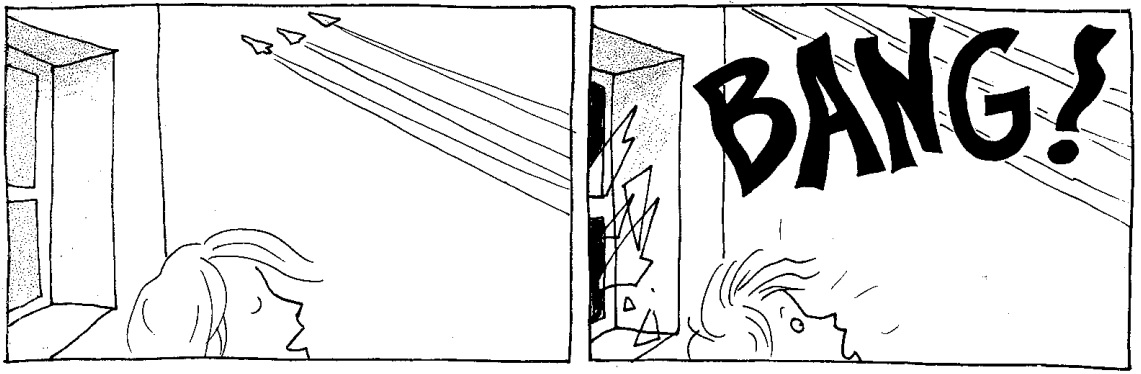
\includegraphics[width=\hsize]{stosswellen/ueberschall.jpg}
\end{center}
\caption{Stosswelle die als "Uberschallknall auftritt. Ausschnitt aus dem Comic "Le Mur du Silence" \, von Jean Pierre Petit\cite{stoss:leMurDeSilence}.}
\label{stosswellen:ueberschall}
\index{Petit, Jean Pierre}
\end{figure}

Stosswellen werden in der Atmosph"are durch verschiedene Ereignisse
hervorgerufen wie etwa durch Explosionen, Blitze oder Flugzeuge,
welche die Schallmauer durchbrechen. Bewegt sich ein Gegenstand
durch ein Medium mit einer Geschwindigkeit, die kleiner ist als die
Wellengeschwindigkeit des Mediums, kann der Gegenstand die Fl"ussigkeit
oder das Gas vorzeitig verdr"angen. Die erzeugte Welle kann sich in
Bewegungsrichtung ausbreiten und Molek"ule \grqq vorwarnen". Dadurch
kann sich der Druck vor dem Gegenstand stetig aufbauen und es entsteht
kein pl"otzlicher Druckanstieg. Bewegt sich der Gegenstand jedoch mit
einer Geschwindigkeit, die schneller ist als die Wellengeschwindigkeit,
kann sich die erzeugte Welle nicht mehr in Bewegungsrichtung ausbreiten
und es entsteht ein abrupter Druckanstieg. Durch diesen Druckanstieg
k"unden sich die Wellen vorg"angig nicht an.

Stosswellen werden durch nicht lineare Partielle Differentialgleichungen
bestimmt. In diesem Kapitel werden wir der Einfachheit halber auf den
speziellen Fall eingehen, dass sich die Welle nur in einer Dimension
ausbreitet, was aufgrund der Nichtlinearit"at trotzdem knifflig genug
ist. {\tt :-)}
\index{nichtlinear}

\section{Transportgleichung}
\index{Transportgleichung}
\lhead{Transportgleichung}
Stosswellen sind L"osungen einer nichtlinearen Transportgleichung. In
diesem Abschnitt sollen die wesentlichen Unterschiede zwischen linearen
und nichtlinearen Transportgleichungen beleuchtet werden.

\subsection{Lineare Transportgleichung}
Bei allen bisher behandelten Partiellen Differentialgleichungen hat es
sich ausschliesslich um lineare Probleme gehandelt, wie zum Beispiel
die Gleichung (\ref{heat:pdgl}) aus dem Kapitel W"armeleitungsgleichung. 
Dabei handelt sich um eine Gleichung der Form

\begin{equation}
	\frac{\partial u}{\partial t}=F(u) \qquad \text{mit} \qquad u = u(x,t) 
	\label{stosswellen:lingl}
\end{equation}

Eine solche Gleichung bezeichnet man als linear, wenn ein System mit
den L"osungen
$u_{1}(x,t)$ und $u_{2}(x,t)$ auch jede Linearkombination
\begin{equation}
	a\cdot u_{1}(x,t) + b \cdot u_{2}(x,t) \qquad \text{mit} \quad a, b = \text{konst.}
	\label{stosswellen:linbed}
\end{equation}
als L"osung besitzt. Dies wird auch als "Uberlagerungssatz oder
Superposition bezeichnet.
\index{Superposition}

Als Beispiel dient eine Transportgleichung im eindimensionalen Fall und bei konstanter Geschwindigkeit $v$. Sie l"asst sich schreiben als
\begin{equation}
	\left\{
	\begin{array}{lcl}
		\frac{\partial u}{\partial t} + v\frac{\partial u}{\partial x} &=& 0 \hspace{1.25cm} \text{f"ur} \quad t>0 \; , \; x \in \mathbb{R} \quad \text{und} \quad v=\text{konst.} \\
		u(x,t\!=\!0) &=& u_{0}(x) \qquad \text{f"ur} \quad x \in \mathbb{R} 
	\end{array} \right.
	\label{stosswellen:lintransp}
\end{equation}
Dass es sich bei der Gleichung (\ref{stosswellen:lintransp}) um eine
Transportgleichung handelt, kann man anhand der Funktion $u_0(x-vt)$
sehen. Sie ist L"osung der Gleichung (\ref{stosswellen:lintransp}),
wie man  durch  Einsetzen nachpr"ufen  kann.  Sie beschreibt einen
Wellenbuckel mit der Form $u_0(x)$, der sich mit Geschwindigkeit v nach
rechts bewegt.

Durch die konstante Geschwindigkeit $v$ l"asst sich die Summe von
\begin{align*}
\frac{\partial u_{1}}{\partial t} + v\frac{\partial u_{1}}{\partial x}&= 0 &\bigg| \cdot a& \\
\frac{\partial u_{2}}{\partial t} + v\frac{\partial u_{2}}{\partial x}&= 0 &\quad \bigg| \cdot b&
\end{align*}
auch schreiben als
\begin{align*}
	\frac{\partial}{\partial t}(au_{1} + bu_{2}) + v\frac{\partial }{\partial x}(au_{1} + bu_{2}) = 0
\end{align*}
womit die Linearit"atsbedingung (\ref{stosswellen:linbed}) erf"ullt ist.

Linearit"at erm"oglicht L"osungen einer Differentialgleichung durch
"Uberlagerung aus einfacheren Teill"osungen aufzubauen. Wird zum Beispiel
die Anfangsbedingung der Gleichung (\ref{stosswellen:lintransp}) mit
$u(x,t\!=\!0)$ durch eine Fourierreihe der Form
\begin{equation}
	u(x,t\!=\!0) = \sum_{k=-\infty}^{+\infty} c_{k} e^{jkx}
\end{equation}
dargestellt, so folgt durch die Linearit"at, dass alle Wellenkomponenten
einzeln und unabh"angig von den anderen integriert werden k"onnen. F"ur
einen sp"ateren Zeitpunkt $u(x,t\!>\!0)$ k"onnen die einzeln berechneten
Komponenten einfach wieder zusammengez"ahlt werden.

Aus diesem Grund werden in der Signaltheorie und der Regelungstechnik
lineare Systeme bevorzugt.

\subsection{Nichtlineare Transportgleichung}

In den meisten str"omungsdynamischen F"allen tritt die Transportgleichung
(\ref{stosswellen:lintransp}) jedoch nicht in linearer Form auf. Die
Nichtlinearit"at entsteht dadurch, dass die Transportgeschwindigkeit
von der transportierten Gr"osse abh"angig ist $v=v(u)$. 

Im speziellen Fall $v\!=\!v(u)\!=\!u$ ergibt sich die \textit{unviskose
Burgersgleichung}\cite{stoss:burgersgleichung}. 
\index{Burgersgleichung}

\begin{equation}
	\left\{
	\begin{array}{lcl}
	\frac{\partial u}{\partial t} + u\frac{\partial u}{\partial x} &=& 0 \hspace{1.25cm} \text{f"ur} \quad t>0 \quad \text{und} \quad x \in \mathbb{R} \\
	u(x,t\!=\!0) &= & u_{0}(x) \qquad \text{f"ur } \quad x \in \mathbb{R} 
	\end{array} \right.
	\label{stosswellen:burgeq}
\end{equation}

H"aufig wird die Gleichung auch in der folgenden, "aquivalenten Form
geschrieben.
\begin{equation}
	\left\{
	\begin{array}{lcl}
		\frac{\partial u}{\partial t} + \frac{1}{2}\frac{\partial u^{2}}{\partial x} &=& 0 \hspace{1.25cm} \text{f"ur} \quad t>0 \quad \text{und} \quad x \in \mathbb{R} \\
		u(x,t\!=\!0) &=& u_{0}(x) \qquad \text{f"ur } \quad x \in \mathbb{R} 
	\end{array} \right.
	\label{stosswellen:burgeq2}
\end{equation}
In dieser Schreibweise kann man erkennen, dass es sich
bei einer Stosswelle um eine eindimensionale hyperbolische
Erhaltungsgleichung\cite{stoss:erhaltungsgleichung} der Form
$\frac{\partial}{\partial t}u + \frac{\partial}{\partial x} f(u) = 0$
mit $f(u) = \frac{1}{2}u^{2}$ handelt.

\subsection{Eigenschaften}
Eine der wichtigsten Eigenschaften einer Stosswelle ist, dass Punkte
eines h"oheren Amplitudenwertes eine h"ohere Geschwindigkeit aufweisen
als Punkte eines tiefen Wertes. Das heisst, dass sich die St"orung nicht
gleichm"assig im Medium vorw"arts bewegt.

Die \textit{unviskose Burgersgleichung} besagt, dass jedes Teilchen
eine konstante Geschwindigkeit beibeh"alt w"ahrend es sich bewegt. Oder
anders ausgedr"uckt, wenn ein Teilchen mit der Geschwindigkeit $u_{0}$
startet, dann wird es zum Zeitpunkt $t$ an der Stelle $x_{0}\!+\!tu_{0}$
immer noch dieselbe Geschwindigkeit haben.
\begin{equation}
u(x_{0}\!+\!tu_{0},t) = u_{0} \qquad \text{f"ur} \quad t \in \mathbb{R^{+}} 
\end{equation} 
Sobald ein Teilchen mit h"oherer Geschwindigkeit zu einem mit einer
tieferen aufgeschlossen hat, entsteht dadurch eine Sprungstelle. An
dieser Stelle "andert sich der Druck sprunghaft. Dies kann mit der
Abbildung \ref{stosswellen:speed} aufgezeigt werden.
\begin{figure}
\begin{center}
\begin{tikzpicture}
	\node at (0,3) {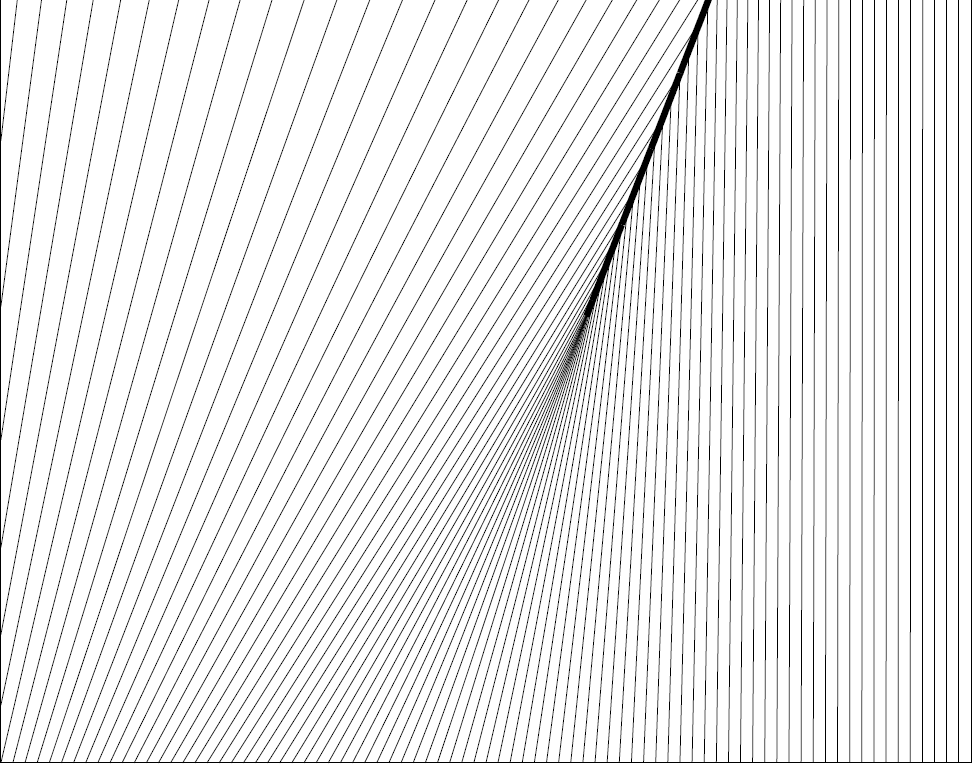
\includegraphics[width=8cm]{stosswellen/speed.png}};
	%Koordinatensystem 
	\draw[line width=1pt,>=latex,->] (-4,-0.15) -- (4.3,-0.15) node[right] {$x$};
	\draw[line width=1pt,>=latex,->] (-4,-0.16) -- (-4,6.5) node[above] {$t$};
\end{tikzpicture}
\end{center}
\caption{Fortbewegungsgeschwindigkeit in der Richtung der Zeit. Als
Anfangsbedingung dient eine Sinushalbwelle. Der dicke Strich entspricht
der Position der Sprungstelle.\cite{stoss:sinusAnfang} 
\label{stosswellen:speed}}
\end{figure}

Aufgrund dieser Sprungstelle entsteht die typische kegelige Form einer
Stosswelle, wie sie in Abbildung \ref{stosswellen:fortpflanzung} links
zu sehen ist.
\begin{figure}
\begin{minipage}[t]{0.45\textwidth}
	\begin{tikzpicture}[scale=1,>=stealth]
	%Koordinatensystem 	
 	\draw[<->] (-0.5,1.2) node[above] {$p$} |- (5,0) node[right] {$x$};
	\draw[->] (-0.5,1.2) |- (5,-1.2) node[right] {$x$};
	\draw[->] (-0.5,1.2) |- (5,-2.4) node[right] {$x$}; 
	\draw[->] (-0.5,1.2) |- (5,-3.6) node[right] {$x$};
	\draw[->] (-0.5,1.2) |- (5,-4.8) node[right] {$x$}; 
	%Wellen einlesen und Plotten
	\draw [color=blue] plot file {stosswellen/data/gut0.txt};
	\draw [color=blue] plot file {stosswellen/data/gut1.txt};
	\draw [color=blue] plot file {stosswellen/data/gut2.txt};
	\draw [color=blue] plot file {stosswellen/data/gut3.txt};
	\draw [color=blue] plot file {stosswellen/data/gut4.txt};
	%Beschriftung 
	\draw (5,0.6) node[] {$t_{0}$};
	\draw (5,-0.6) node[] {$t_{1}>t_{0}$};
	\draw (5,-1.8) node[] {$t_{2}>t_{1}$};
	\draw (5,-3) node[] {$t_{3}>t_{2}$};
	\draw (5,-4.2) node[] {$t_{4}>t_{3}$};			
\end{tikzpicture}
\end{minipage}
\hfill
\begin{minipage}[t]{0.45\textwidth}
\begin{tikzpicture}[scale=1,>=stealth]
	%Koordinatensystem 	
 	\draw[<->] (-0.5,1.2) node[above] {$p$} |- (5,0) node[right] {$x$};
	\draw[->] (-0.5,1.2) |- (5,-1.2) node[right] {$x$};
	\draw[->] (-0.5,1.2) |- (5,-2.4) node[right] {$x$}; 
	\draw[->] (-0.5,1.2) |- (5,-3.6) node[right] {$x$};
	\draw[->] (-0.5,1.2) |- (5,-4.8) node[right] {$x$}; 
	%Wellen einlesen und Plotten
	\draw [color=blue] plot file {stosswellen/data/aus0.txt};
	\draw [color=blue] plot file {stosswellen/data/aus1.txt};
	\draw [color=blue] plot file {stosswellen/data/aus2.txt};
	\draw [color=blue] plot file {stosswellen/data/aus3.txt};
	\draw [color=blue] plot file {stosswellen/data/aus4.txt};
	%Beschriftung 
	\draw (5,0.6) node[] {$t_{0}$};
	\draw (5,-0.6) node[] {$t_{1}>t_{0}$};
	\draw (5,-1.8) node[] {$t_{2}>t_{1}$};
	\draw (5,-3) node[] {$t_{3}>t_{2}$};
	\draw (5,-4.2) node[] {$t_{4}>t_{3}$};	
\end{tikzpicture}
\end{minipage}
\caption{Fortbewegung einer Sinushalbwelle mit fortlaufender Zeit.
Links:
Schematische Darstellung einer Stosswelle mit einer
Sinushalbwelle als Anfangsbedingung.
Rechts:
Numerische L"osung zur selben Anfangsbedingung mittels
Leapfrog-Schema, eine nicht lineare Instabilit"at bei der Sprungstelle
l"asst das Bild ausreissen.
\label{stosswellen:fortpflanzung}
}
\end{figure}


\section{Problemstellung}

Die Wellenausbreitung der \textit{unviskosen Burgersgleichung}
(\ref{stosswellen:burgeq}) soll mittels eines numerischen
L"osungsverfahrens simuliert werde k"onnen. Wir verwenden daf"ur die
\textit{Finite Differenzen Methode} auch als \textit{Gitterpunktmethode}
bekannt. Als Anfangsbedingung $u(x,t\!=\!0)$ sollen verschiedene
Wellenformen wie z.B. eine Sinushalbwelle oder ein Gaussglocke dienen. 

\section{Diskretisierung}
\lhead{Diskretisierung}
Zur Diskretisierung teilen wir die $x$-Achse im Intervall $[0,1]$ in $N$
Punkte $x_{n}$. Die $t$-Achse wird ebenfalls in eine endliche Anzahl
Punkte $t_{m}$ im Intervall $[0,M]$ unterteilt. Die Intervallgrenze
$M$ kann, je nach Dauer der Simulation sehr unterschiedlich gew"ahlt
werden und wird deshalb nicht konkret gesetzt. Die Funktion $u(x,t)$
wird ersetzt durch die Werte von $u$ auf den Gitterpunkten, wir schreiben
\begin{equation*}
	u(x,t) \Rightarrow u(x_{n},t_{m}) \qquad \text{mit} \quad 0 \leq n \leq N \, , \, 0\leq m \leq M.
\end{equation*}
Die Anfangsbedingung $u(x_n,t_0)$ muss "uber das gesamte $x$-Intervall
bekannt sein. Das $x$-Intervall des darauffolgenden Zeitschrittes
$u(x_n,t_1)$ wird dann aus den Werten der Anfangsbedingung berechnet. So
m"ussen alle Gitterpunkte eines Zeitpunktes $t_m$ iterativ aus den Werten
der vorg"angigen Zeitschritten berechnet werden k"onnen. 

\subsection{Upstream-Schema}
\index{Upstream-Schema}
Da es sich beim Problem um eine Differentialgleichung handelt, muss man
auch den Differentialquotient auf diskrete Werte anwenden k"onnen. Es ist
naheliegend, dass man bei der bekannten Formel der partiellen Ableitung
an der Position $x_{0}$
\begin{equation}
	\frac{\partial u}{\partial x} = \lim\limits_{\Delta x \to 0} \frac{{u(x_{0}}\!+\!\Delta x,t)-u(x_{0},t)}{\Delta x}
\end{equation}
einfach die $\lim\limits_{\Delta x \to 0}$ Bedingung wegl"asst. So erh"alt man f"ur die r"aumliche Ableitung
\begin{equation}
	\frac{\partial u}{\partial x} \Bigg|_{x_{n}} \approx \frac{u(x_{n\!+\!1},t_{m})-u(x_{n},t_{m})}{\Delta x}
	\label{stosswellen:upsteamort}
\end{equation}
und f"ur die zeitliche Ableitung
\begin{equation}
	\frac{\partial u}{\partial t} \Bigg|_{x_{n}} \approx \frac{u(x_{n},t_{m\!+\!1})-u(x_{n},t_{m})}{\Delta t}.
	\label{stosswellen:eulerschritt}
\end{equation}

Den Zeitschritt (\ref{stosswellen:eulerschritt}) bezeichnet man als
\textit{Euler-} oder \textit{Forward-}Schritt, da er vom bekannten
Zeitniveau $m$ vorw"arts (in die Zukunft) zeigt. Deshalb heisst diese
Methode auch \textit{Upstream-}Schema. Das heisst, weder die zeitliche
noch die r"aumliche Ableitung ist symmetrisch. Dies kann das Resultat
verf"alschen wie in Abbildung \ref{stosswellen:eulerableitung} zu sehen
ist. F"ur den n"achsten Zeitschritt ben"otigen wir die Ableitung der
Funktion $u(x,t)$ an der Stelle $x$. Da wir diskret rechnen, approximieren
wir diese mit der Differenz (\ref{stosswellen:upsteamort}). Da nur zwei
Werte verwendet werden, w"urde die korrekte Approximation dazwischen
liegen. Jedoch liegt dort kein Gitterpunkt, deshalb setzen wir das
Resultat auf den n"achstliegenden Punkt rechts davon. Dadurch erzeugen
wir einen ungewollten Rechtsdrift. Man k"onnte das Resultat auch auf
den linken Punkt setzen, so w"urde einfach ein Linksdrift entstehen.

\begin{figure}[h]
\begin{center}
	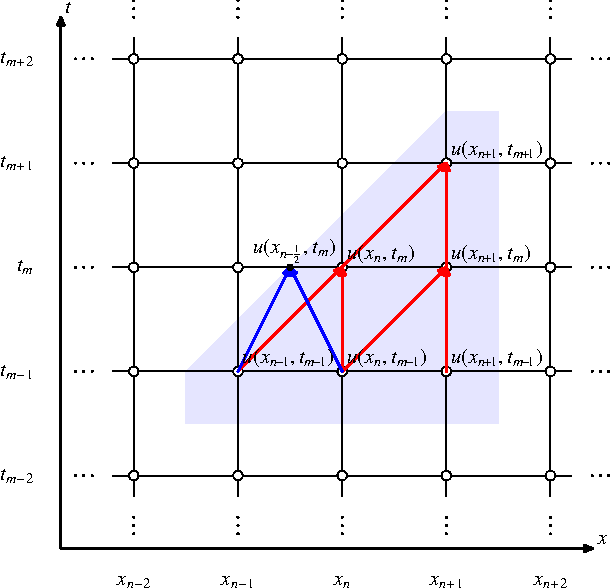
\includegraphics[width=8cm]{stosswellen/stoss-2.pdf}
\end{center}
\caption{Ableitung mittels des \textit{Upstream-}Schemas: F"ur
den n"achsten Zeitschritt wird die Ableitung an der aktuellen und
vorherigen $x$-Position verwendet. Aus diesem Grund w"are die korrekte
Position zwischen den beiden Werten (blaue Pfeile). Da diese nicht auf
das Gitterraster passen, werden sie auf den Gitterpunkt rechts davon
gesetzt. So entsteht ein ungewollter Rechtsdrift in der Rechnung.
\label{stosswellen:eulerableitung}}
\end{figure}


\subsection{Leapfrog-Schema}
\label{stosswellen:kleapfrog}
\index{Leapfrog-Schema}
Da wir keinen Drift in unserer Simulation wollen, ist das obige Verfahren
f"ur uns nutzlos. Wir verwenden stattdessen das \textit{Leapfrog-}Schema,
dieses ist r"aumlich und zeitlich zentriert. Die partiellen Ableitungen
lauten 
\begin{align}
	\frac{\partial u}{\partial x} \Bigg|_{x_{n}} &\approx \frac{u(x_{n\!+\!1},t_{m})-u(x_{n\!-\!1},t_{m})}{2\Delta x}
	\label{stosswellen:leapfrog1} \\
	\frac{\partial u}{\partial t} \Bigg|_{x_{n}} &\approx\frac{u(x_{n},t_{m\!+\!1})-u(x_{n},t_{m\!-\!1})}{2\Delta t}.
	\label{stosswellen:leapfrog2}
\end{align}

Im Gegensatz zum \textit{Upstream-}Schema werden hier f"ur den n"achsten
Zeitschritt die Terme zum Zeitpunkt $t_{n\!-\!1}$ verwendet. Die
Bezeichnung \textit{Leapfrog} (umgangssprachlich Bockspringen) kommt
vom speziellen Zeitsprung. (Abbildung \ref{stosswellen:leapfrogjump})

\begin{center}
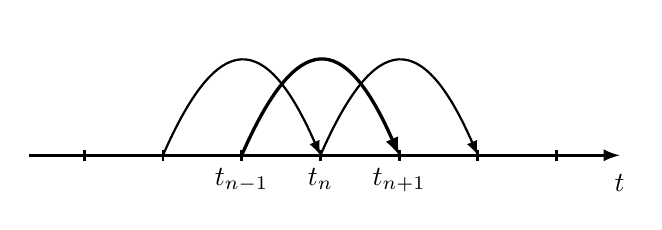
\begin{tikzpicture}[domain=-2.3:4.3, line width=1pt]
	%%Koordinatensystem
		\draw[line width=1pt,>=latex,->] (-2.7,0) -- (4.8,0) node[below=3pt] {$t$};
	%%Gitterpunkte
	\foreach \x in {-2,-1,3,4}
		\draw [line width=1pt] (\x,-2pt) -- (\x,2pt);
	\foreach \x in {0}
		\draw [line width=1pt] (\x,-2pt) -- (\x,2pt) node[below=3pt] {$t_{n-1}$};
	\foreach \x in {1}
		\draw [line width=1pt] (\x,-2pt) -- (\x,2pt) node[below=3pt] {$t_{n}$};
	\foreach \x in {2}
		\draw [line width=1pt] (\x,-2pt) -- (\x,2pt) node[below=3pt] {$t_{n+1}$};																
	%%Pfeile
	\draw [line width=0.8pt,>=latex,->] (-1,0) .. controls(-0.3,1.6) and (0.3,1.6).. (1,0); 
	\draw [line width=1.2pt,>=latex,->] (0,0) .. controls(0.7,1.6) and (1.3,1.6).. (2,0); 		
	\draw [line width=0.8pt,>=latex,->] (1,0) .. controls(1.7,1.6) and (2.3,1.6).. (3,0); 
%			 
%	\draw [>=to,<-] (1,0) arc (0:180:1);	
%	\draw [very thick,>=to,<-] (2,0) arc (0:180:1);
%	\draw [>=to,<-] (3,0) arc (0:180:1);
\end{tikzpicture}

\captionof{figure}{Darstellung des Leapfrog Sprung, f"ur den Zeitschritt
$t_{n\!+\!1}$ wird $t_{n\!-\!1}$ ben"otigt.}
\label{stosswellen:leapfrogjump}
\end{center}

Das \textit{Leapfrog-}Schema verkn"upft immer drei aufeinanderfolgende
Werte miteinander. Zur Startzeit ist in der Anfangsbedingung f"ur die
Zeitableitung nur ein Wert verf"ugbar. Daher m"ussen f"ur den Startschritt
zus"atzliche  Werte  definiert werden. Wir verwenden folgende Konvention:
$u(x,t_{})=u(x,t_{1})$. Zudem k"onnen wir die "aussersten Werte des
$x$-Intervalls nicht berechnen. Sie werden deshalb auf einen fixen Wert
gesetzt. Um durch dieses Vorgehen keine Verf"alschung der Simulation
zu erzeugen, darf das Geschehen nicht direkt am Rand der $x$-Achse
stattfinden. 

Die Gleichungen (\ref{stosswellen:leapfrog1}) und
(\ref{stosswellen:leapfrog2}) k"onnen nun in die Ausgangsgleichung
(\ref*{stosswellen:burgeq}) eingesetzt werden. Dann erh"alt man
\begin{align}
	0 &= \frac{\partial u}{\partial t} + u\frac{\partial u}{\partial x} \notag 	 \\
	0 &= \frac{u(x_{n},t_{m\!+\!1})-u(x_{n},t_{m\!-\!1})}{2\Delta t} + u(x_{n},t_{m}) \frac{u(x_{n\!+\!1},t_{m})-u(x_{n\!-\!1},t_{m})}{2\Delta x} \quad &\bigg| \cdot 2\Delta t \notag \\
	0 &= u(x_{n},t_{m\!+\!1})-u(x_{n},t_{m\!-\!1}) +\frac{\Delta t}{\Delta x}\Bigg( u(x_{n},t_{m}) \Big(u(x_{n\!+\!1},t_{m})-u(x_{n\!-\!1},t_{m})\Big) \Bigg) \notag \\
	u(x_{n},t_{m\!+\!1}) &= u(x_{n},t_{m\!-\!1}) -\frac{\Delta t}{\Delta x}\Bigg( u(x_{n},t_{m}) \Big(u(x_{n\!+\!1},t_{m})-u(x_{n\!-\!1},t_{m})\Big) \Bigg)
	\label{stosswellen:unext}
\end{align}
Um den Wert $u(x_{n},t_{m\!+\!1})$ berechnen zu k"onnen,
ben"otigen wir die Werte $u(x_{n},t_{m\!-\!1})$, $u(x_{n},t_{m})$,
$u(x_{n\!-\!1},t_{m})$ und $u(x_{n\!+\!1},t_{m})$. Dies ist in Abbildung
\ref{stosswellen:leapfrog} dargestellt.
\begin{figure}
\begin{center}
	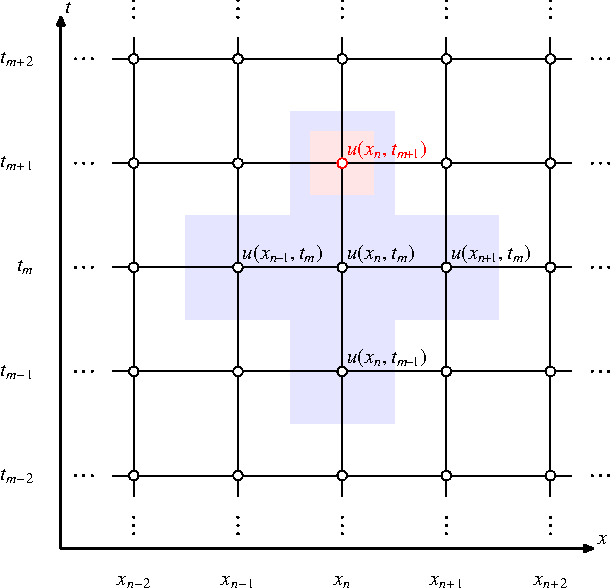
\includegraphics[width=8cm]{stosswellen/stoss-1.pdf}
\end{center}
\caption{Ableitung mittels des \textit{Leapfrog-}Schemas: Durch
die r"aumliche und zeitliche Zentrierung k"onnen wir den n"achsten
Zeitschritt berechnen, ohne einen Drift zu erzeugen. Zu sehen ist, dass
die Intervallgrenzen f"ur den n"achsten Zeitschritt nicht berechnet
werden k"onnen. 
\label{stosswellen:leapfrog}}
\end{figure}



\subsection{Courant-Zahl}
\index{Courant-Zahl}
Ebenfalls sehr wichtig in der Gleichung (\ref{stosswellen:unext}) ist
das Verh"altnis von $\frac{\Delta t}{\Delta x}$. Dieses wird "uber die
Courant-Zahl, auch CFL-Zahl\cite{stoss:cfl} genannt, bestimmt. Sie gibt
die dimensionslose Verschiebung pro Zeitschritt an und ist definiert
durch: 
\[
c=v\frac{\Delta t}{\Delta x}
\]
wobei $c$ die Courant-Zahl und $v$ die Geschwindigkeit
darstellt. Die CFL-Bedingung besagt, dass das \textit{Euler-}
oder \textit{Leapfrog-}Verfahren nur f"ur Courant-Zahlen $c\!<\!1$
stabil ist. Bei unseren Simulationen der Stosswelle wird $v\!=\!u$
angenommen. F"ur die gr"osste Courant-Zahl $c_{max}$ f"allt $v$ somit weg,
da $v_{max}\!=\!u_{max}\!=\!1$ ist.


\section{Nichtlinearit"at und Computational Mode}
\lhead{Nichtlinearit"at und Computational Mode}
\label{stosswellen:nichtlinearit"at}
\subsection{Computational Mode}
Im Abschnitt \ref{stosswellen:kleapfrog} haben wir erkannt, dass wir ein
zentriertes Verfahren f"ur den Differentialquotienten ben"otigen. Jedoch
ist das \textit{Leapfrog-}Schema auch nicht fehlerfrei. So k"onnen
neben den gew"unschten "physikalischen" \, L"osungen auch noch \grqq
k"unstliche" \, L"osungen auftreten. Diese zus"atzlichen L"osungen werden
\textit{Computational Mode} genannt. Diesen negativen Effekt werden wir
anhand zweier Beispielen aufzeigen.

\subsection{Konstante Funktion}
Wir wollen folgende lineare Differentialgleichung aufl"osen.
\begin{equation}
	\frac{d u }{dx} = 0
\end{equation}
Diese Gleichung hat die eindeutige L"osung $u\! =\! \text{konst.}
$ Wenn wir diese Gleichung numerisch l"osen wollen, m"ussen wir sie
diskretisieren. Als erstes verwenden wir das \textit{Upstream-}Schema.
\begin{align}
	\frac{u_{n+1}-u_n}{\Delta x}  &= 0 &\bigg| \cdot \Delta x \; \text{,} \; +u_n \notag \\
	u_{n+1} &= u_n
\end{align}
Diese L"osung stimmt mit dem algebraischen Resultat "uberein. Nun wenden
wir das \textit{Leapfrog-}Schema an.
\begin{align}
	\frac{u_{n+1}-u_{n-1}}{2 \Delta x}  &= 0 &\bigg| \cdot 2 \Delta x \; \text{,} \; +u_{n-1} \notag \\
	u_{n+1} &= u_{n-1}
\end{align}
Diese L"osung kann, muss aber nicht mehr mit dem algebraischen Resultat
"ubereinstimmen. Sie besagt nur, dass alle geraden und ungeraden
Variablen konstant sein m"ussen. Es sind daher die folgende beiden
L"osungen m"oglich:
\begin{center}
	\begin{tabular}{c|c|c|c|c|c|c}

		...	&	{$x_{n-2}$} 	& {$x_{n-1}$} 	& {$x_{n}$} & {$x_{n+1}$} & {$x_{n+2}$}	&	... \\
		\hline
		1	&	1	& 	1	&	1	&	1	&	1	&	1 \\
		\hline
		$\pm$ 1	&	1	& 	-1	&	1	&	-1	&	1	&	$\pm$ 1 \\
	\end{tabular}
\end{center}
Die erste L"osung ist die korrekte L"osung, denn nur dort gilt
$u\!=\! \text{konst.}$ Die zweite L"osung ist der "k"unstlich" \,
erzeugte \textit{Computional Mode}.
\index{Computational Mode}

\subsection{Exponentialfunktion}
Als zweites Beispiel wollen wir folgende lineare Differentialgleichung
aufl"osen. 
\begin{equation}
	\frac{d u }{dx} = -k \cdot u
\end{equation} 
Aus der Analysis kennen wir das Resultat f"ur diese Gleichung. Es lautet:
$u = e^{-kx}$. Wir wenden erneut das \textit{Leapfrog-}Schema an.
\begin{align}
	\frac{u_{n+1} - u_{n-1}}{2 \Delta x} &= -k u_n  \notag\\
	u_{n+1}& = u_{n-1} - 2 \Delta x k u_n
	\label{stosswellen:cm_bsp2}
\end{align}
Dies ist ein Beispiel einer Differenzengleichung, welche mit Hilfe von
Eigenwerten und Eigenvektoren gel"ost werden kann. \cite{stoss:linAlg} 
\begin{equation}
	\begin{pmatrix}u_{n+1}\\u_n\end{pmatrix}
	=
	\begin{pmatrix}-2k\Delta x u_n+u_{n-1}\\u_n\end{pmatrix}
	=
	\begin{pmatrix}
	-2k \Delta x & 1 \\
	1 & 0
	\end{pmatrix}
	\begin{pmatrix}u_n\\u_{n-1}\end{pmatrix}
	=
	A
	\begin{pmatrix}u_n\\u_{n-1}\end{pmatrix}
	\label{fibonaccirekursion}
\end{equation}

Die Matrix
\[
A = \begin{pmatrix}	-2k \Delta x & 1\\	1 & 0\end{pmatrix}
\]
hat das charakteristische Polynom
\begin{align*}
 	\det(A-\lambda I)&=\left|\begin{matrix}-2k \Delta x-\lambda&1\\1&-\lambda\end{matrix}\right|\\
 	&= (-2k \Delta x - \lambda) (-\lambda) -1=\lambda^2 + 2k\Delta x \lambda-1
\end{align*}
mit den L"osungen
\begin{align}
\lambda_\pm &= \frac{-2k \Delta x \pm \sqrt{4k^2 \Delta x^2 + 4}}{2} \notag \\
\lambda_+ &= -k \Delta x + \sqrt{k^2 \Delta x^2 + 1} < 1 \\
\lambda_- &= -k \Delta x - \sqrt{k^2 \Delta x^2 + 1} < -1.\\
\end{align}
Wie man in Abbildung \ref{stosswellen:lamda} sehen kann, ist der Betrag
von $\lambda_+$ kleiner als 1, wohingegen $\lambda_-$ einen Betrag
gr"osser 1 hat.
\begin{figure}
	\begin{center}
		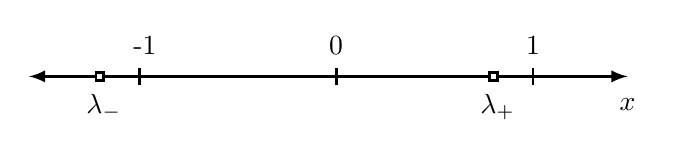
\begin{tikzpicture}[line width=1pt]
			%%Koordinatensystem
			\draw[line width=1pt,>=latex,<->] (-1.4,0) -- (6.2,0) node[below=4pt] {$x$};
		
			%%Gitterpunkte				
			\foreach \x in {0}
				\draw [line width=1pt] (\x,-3pt) -- (\x,3pt) node[right = 2pt, above=1pt] {-1};		
			\foreach \x in {2.5}
				\draw [line width=1pt] (\x,-3pt) -- (\x,3pt) node[above=1pt] {0};
			\foreach \x in {5}
				\draw [line width=1pt] (\x,-3pt) -- (\x,3pt) node[above=1pt] {1};												
			%%Pfeil 
			\draw [fill=white] (-0.55,-0.05) rectangle (-0.45,0.05) node[below=4pt] {$\lambda_-$};
			\draw [fill=white] (4.45,-0.05) rectangle (4.55,0.05) node[below=4pt] {$\lambda_+$};
		\end{tikzpicture}
		\caption{Anordnung von $\lambda_\pm$ auf dem Zahlenstrahl}
		\label{stosswellen:lamda}
	\end{center}
\end{figure}
Aus den Eigenwerten $\lambda_\pm$ folgen die Eigenvektoren 
\begin{align}
 	\vec v_+=\begin{pmatrix}-k\Delta x + \sqrt{k^2\Delta x^2 + 1}\\ 1\end{pmatrix} &\approx \begin{pmatrix} 1 \\ 1 \end{pmatrix} \\
 	\qquad
 	\vec v_-=\begin{pmatrix}-k\Delta x - \sqrt{k^2\Delta x^2 + 1}\\ 1\end{pmatrix} &\approx \begin{pmatrix} -1 \\ 1 \end{pmatrix} 
\end{align}
Nun k"onnen wir die L"osung der Differenzengleichung aufschreiben. Die Konstanten $a$ und $b$ kommen durch die Anfangsbedingung zustande.
\begin{align}
	\begin{pmatrix} u_{n+1} \\ u_n \end{pmatrix}  &= a \lambda_+^n \vec v_+ +  b \lambda_-^n \vec v_- \\
	u_n & =  \underbrace{a \lambda_+^n}_{\text{physikalische L"osung}} + \underbrace{ b \lambda_-^n}_{\text{Computational Mode}} 
	\label{stosswellen:cmexpo}
\end{align}
Der Term $a\lambda_+^n$ nimmt exponentiell ab, da $|\lambda_-|>1$ wird
der Term $b\lambda_-^n$ jedoch exponentiell anwachsen. Dadurch wird das
Resultat \grqq explodieren" \ und nicht mit der algebraischen L"osung
"ubereinstimmen.

Wichtig ist, dass der \textit{Computational Mode} ein reines numerisches
Problem ist, welches bei linearen und nichtlinearen Gleichungen auftreten
kann. Die \grqq k"unstlich" \, erzeugte L"osung muss aber nicht immer
eine Instabilit"at hervorrufen. Falls beide Eigenwerte $\lambda_\pm$
einen Betrag $\leq$ 1 haben, bleibt die L"osung stabil. Da ein Computer
nur rationale Zahlen genau aufl"osen kann, haben irrationale Zahlen
immer eine minimal kleine Abweichung. Aufgrund dieser Abweichung kann
der \textit{Computational Mode} in der Numerik nicht verhindert werden.


\subsection{Nichtlineare Instabilit"at}
Die analytische L"osung einer Stosswelle wird in Abbildung
\ref{stosswellen:fortpflanzung} links illustriert. Wenn wir die
\textit{unviskose Burgersgleichung} (\ref{stosswellen:burgeq}) numerisch
mit dem \textit{Leapfrog-}Schema Kap. \ref{stosswellen:kleapfrog}
l"osen, bekommen wir aber eine L"osung, wie sie in Abbildung
\ref{stosswellen:fortpflanzung} rechts zu sehen ist. Die
numerische Simulation ist offenbar instabil, man spricht von der
\textit{nichtlinearen Instabilit"at}. In diesem Abschnitt soll gezeigt
werden, dass die Nichtlinearit"at der \textit{Burgersgleichung} das
Auftreten des \textit{Computational Mode} beg"unstigt. 

Wir nehmen einfachheitshalber an, dass sich die $x$-Abh"angigkeit von
$u(x,t)$ zu jedem Zeitpunkt durch eine Sinus-Reihe darstellen l"asst.
\begin{equation}
	u(x,t) = \sum_{k=1}^{\infty} U_{k}(t) \sin(2\pi kx) \qquad \text{mit} \quad x \in[0;1]
	\label{stosswellen:sinreihe}
\end{equation} 

$U_{k}(t)$ ist die zeitabh"angige Amplitude und $k$ die Wellenzahl. 
Die Funktion (\ref{stosswellen:sinreihe}) hat folgende Partielle Ableitungen:
\begin{align*}
	\frac{\partial u}{\partial t}&=
	\sum_{k=1}^{\infty} \sin(2\pi k x) \frac{\partial U_{k}(t)}{\partial t}
\\
	\frac{\partial u}{\partial x}&=
	\sum_{k=1}^{\infty} 2\pi k U_{k}(t) \cos(2\pi k x) 
\end{align*}

Wir setzen diese in die Gleichung (\ref{stosswellen:burgeq}) ein und erhalten:
\begin{equation}
	\sum_{k=1}^{\infty}\sin(2\pi k x) \frac{\partial U_{k}(t)}{\partial t} + \sum_{k_{1}=1}^{\infty} U_{k_{1}}(t) \sin(2\pi k_{1}x) \cdot \sum_{k_{2}=1}^{\infty}2\pi k_{2} U_{k_{2}}(t) \cos (2\pi k_{2} x)
	= 0
	\label{stosswellen:bursin}
\end{equation}
Die r"aumliche Ableitung der Gleichung (\ref{stosswellen:bursin}) l"asst
sich weiter vereinfachen auf:
\begin{align}
	u\frac{\partial u}{\partial x} &= 
	\sum_{k_{1}=1}^{\infty} \sum_{k_{2}=1}^{\infty} 2 \pi k_{2} U_{k_{1}}(t) U_{k_{2}}(t) \sin (2\pi k_{1}x) \cos (2\pi k_{2}x) \notag\\
	&= \sum_{k_{1}=1}^{\infty} \sum_{k_{2}=1}^{\infty} \pi k_{2} U_{k_{1}}(t) U_{k_{2}}(t) (\sin (2\pi (k_{1}+k_{2})x) + \sin(2\pi (k_{1}-k_{2})x)
\end{align}

Durch die Wechselwirkung zweier Wellen mit den Wellenzahlen $k_{1}$
und $k_{2}$ ist eine Summe aus zwei neuen Wellen mit den Wellenzahlen
$k_{1}\!+\!k_{2}$ und $k_{1}\!-\!k_{2}$ entstanden. Durch die
Nichtlinearit"at $u\frac{\partial u}{\partial x}$ k"onnen also Wellenmoden
entstehen, die vorher noch nicht vertreten gewesen sind. Dies ist die
Ursache f"ur die \textit{nichtlineare Instabilit"at}. Da  \grqq neue"
\, L"osungen entstehen, werden auch L"osungen des \textit{Computational
Mode} entstehen. Wie wir in \ref{stosswellen:cmexpo} gesehen haben,
k"onnen diese L"osungen exponentiell ansteigen. Bei der Sprungstelle
passiert genau dies und deshalb bricht dort das Signal aus. 

\subsection{Aliasing}
Man kann die verst"arkte Anregung des \textit{Computational Mode} auch
als eine Folge von \textit{Aliasing} verstehen. Wird die $x$-Achse durch
eine endliche Anzahl von Punkten im Abstand von $\Delta x$ diskretisiert,
k"onnen nur Wellen bis zu einer minimalen Wellenl"ange von $\lambda_{min}
\!=\! \frac{2 \pi}{k}\! = \! 2 \Delta x$ aufgel"ost werden. Daraus folgt
die gr"osstm"ogliche Wellenzahl:
\begin{equation}
	k_{max} = \frac{\pi}{\Delta x}\,.
\end{equation}

Wenn nun die nichtlineare Wechselwirkung versucht eine Welle zu erzeugen,
welche eine gr"ossere Wellenzahl als $k_{max}$ hat, kann diese durch
das Gitter nicht ad"aquat beschrieben werden. Die Welle erscheint durch
'Schwebung' als eine l"angere Welle. 

Dies kann durch ein einfaches Beispiel illustriert werden. Wir definieren
\begin{equation}
	\phi_{k} = \cos (kx) \qquad \text{mit} \quad k>k_{max}.
\end{equation}
In der Euler-Form dargestellt:
\begin{equation}
	\phi_{k} = \frac{1}{2}(e^{jkx} + e^{-jkx}).
	\label{stosswellen:eulercos}
\end{equation}
Definiert man 
\begin{equation*}
	k_{a} := 2k_{max} - k \qquad \Rightarrow \qquad k = 2k_{max} - k_{a},
\end{equation*}
so folgt f"ur (\ref{stosswellen:eulercos})
\begin{equation*}
	\phi_{k} = \frac{1}{2}(e^{j2k_{max}x}e^{-jk_{a}x} + e^{-j2k_{max}x}e^{jk_{a}x})
\end{equation*}

Da die Funktion nur auf den diskreten Gitterpunkten $x_{n}\! =\! n \Delta
x$ definiert ist, verschwinden die Terme mit $k_{max}$ gem"ass
\begin{equation*}
	 e^{j2k_{max}x} \bigg|_{\substack{x = n \Delta x \\ k_{max} = \frac{\pi}{\Delta x}}} = e^{j2\pi n} = 1 \qquad (n\!=\!1,2,3,..)
\end{equation*}
Dadurch wird $\phi_{k}$ f"alschlicherweise dargestellt als 
\begin{equation}
	\phi_{k} = \frac{1}{2}(e^{-jk_{a}x} + e^{jk_{a}x}) = \cos (k_{a}x) \qquad \text{mit} \quad k_{a}<k_{max}. 
\end{equation}
Da die Wellenzahl $k_{a}$ kleiner als $k_{max}$ ist, kann diese
Welle, im Gegensatz zur urspr"unglichen, auf dem Gitter dargestellt
werden. Eine Veranschaulichung des Aliasing-Fehlers wird in Abbildung
\ref{stosswellen:aliasing} dargestellt.

\begin{figure}
\begin{minipage}{0.45\textwidth}
\
	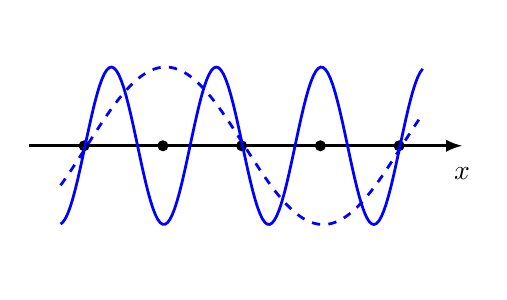
\begin{tikzpicture}[domain=-0.3:4.3]
		%Koordinatensystem
		\fill [fill=white] (0,-1.6) rectangle (2.5,1.5);
		\draw[line width=1pt,>=latex,->] (-0.7,0) -- (4.8,0) node[below=4pt] {$x$};
		%Gitterpunkte
		\foreach \x in {0,1,2,3,4}
			\fill (\x,0) circle[radius=2pt];
		%Funktion
		\draw[color=blue, samples=150, line width=1pt] plot (\x,{sin(4.7123889804*\x r-pi)}) ;
		\draw[color=blue, samples=150, dashed, line width=1pt] plot (\x,{sin(1.5707963268*\x r-pi)}) ;
	\end{tikzpicture}
\end{minipage}
\hfill
\begin{minipage}{0.45\textwidth}
	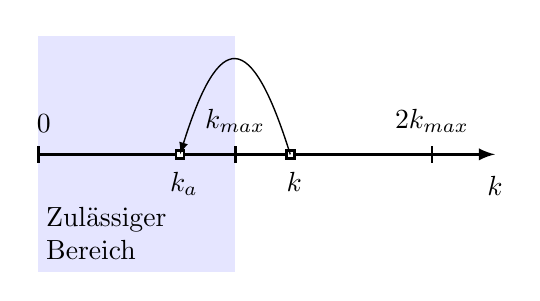
\begin{tikzpicture}[line width=1pt]
		%Zulaessiger Bereich
		\definecolor{lightgray}{rgb}{0.9,0.9,1}
		\fill [fill=lightgray] (0,-1.5) rectangle (2.5,1.5);
		
		%Koordinatensystem
		\draw[line width=1pt,>=latex,->] (0,0) -- (5.8,0) node[below=4pt] {$k$};
		\node[text width=2cm] at (1.1,-1) {Zul\"assiger Bereich};
		
		%Gitterpunkte				
		\foreach \x in {0}
			\draw [line width=1pt] (\x,-3pt) -- (\x,3pt) node[right = 2pt, above=1pt] {$0$};		
		\foreach \x in {2.5}
			\draw [line width=1pt] (\x,-3pt) -- (\x,3pt) node[above=1pt] {$k_{max}$};
		\foreach \x in {5}
			\draw [line width=1pt] (\x,-3pt) -- (\x,3pt) node[above=1pt] {$2k_{max}$};												
		%Pfeil 
		\draw [fill=white] (1.75,-0.05) rectangle (1.85,0.05) node[below=4pt] {$k_{a}$};
		\draw [fill=white] (3.15,-0.05) rectangle (3.25,0.05) node[below=4pt] {$k$};
		\draw [line width=0.5pt,>=latex,<-] (1.8, 0) .. controls(2.3,1.6) and (2.7,1.6).. (3.2, 0);
	\end{tikzpicture}
\end{minipage}
\caption{Illustration des Aliasing-Fehlers im Zeitbereich und im
\index{Aliasing-Fehler}
Spektralen Raum.
Links: Eine Welle mit Wellenl"ange $\frac{4 \Delta x}{3}$ wird
f"alschlicherweise als eine Welle mit Wellenl"ange $4\Delta x$ angezeigt.
Rechts: Bei einer Welle mit einer Wellenzahl $k\!>\!k_{max}$ wird die
Wellenzahl f"alschlicherweise als $k_{a}\!=\!2k_{max}\!-\!k$ angenommen.
\label{stosswellen:aliasing}	
}
\end{figure}
 

\subsection{Filter}
\label{stosswellen:loesung}
\index{nichtlineare Instabilitat@nichtlineare Instabilit\"at}
Die theoretisch exakte L"osung zur Behebung der \textit{nichtlinearen
Instabilit"at} folgt aus der vorherigen Definition. Wenn man bei jedem
Zeitschritt alle Wellen mit einer Wellenzahl $k > \frac{k_{max}}{2}$
eliminiert, kann kein Aliasing entstehen. Denn jede neu entstandene
Welle mit $k_{1}\!+\!k_{2}$ kann auf dem Gitter aufgel"ost werden. 

Um eine Eliminierung der Wellen zu erm"oglichen, muss nach jedem Schritt
das Signal mit einer Fouriertransformation in den Spektralbereich
transformiert werden. Dort kann man die zu hohen Frequenzen
herausfiltern. Anschliessend wird das Signal r"ucktransformiert. Da diese
Methode viel zu aufw"andig ist, verwendet man in der Praxis digitale
Filter und verzichtet auf die Transformationen.

Ein relativ einfaches Filter, welches auf das $x$-Intervall angewandt
wird, lautet:
\begin{equation}
\tilde{u}(x_n,t) = u(x_n,t_m) + \alpha \Big(u(x_{n-1},t_m)-2 u(x_n,t_m) + u(x_{n+1},t_m)\Big) \qquad \text{mit} \quad \alpha \in (0;1)
\end{equation}

Dieses Filter ist bekannt unter dem Namen
\textit{Robert-Asselin-Time-Filter}\cite{stoss:filter}. Wir wenden es
\index{Robert-Asselin-Time-Filter}
jedoch nicht auf die Zeitvariable $t$ an, sondern nach jedem Zeitschritt
auf alle $x$-Werte, gegebenenfalls auch mehrmals hintereinander. Dadurch
werden grosse "Anderungen in der Amplitudenh"ohe gegl"attet. Jede
Filterung vergr"ossert nat"urlich den Rechenaufwand pro Zeitschritt und
deshalb sollte nur so stark gefiltert werden wie n"otig. 


Eine andere Methode die \textit{nichtlinearen Instabilit"at} zu
eliminieren liegt darin, das Problem von der physikalischen Seite her zu
betrachten. Da es sich bei unserer Stosswelle um eine Erhaltungsgleichung
handelt, bleibt die Energie "uber das gesamte Intervall erhalten. Das
heisst, Werte an Punkten die zur aktuellen Zeit rechts von der
Sprungstelle liegen, k"onnen im n"achsten Schritt nicht gr"osser
sein als das aktuelle Maximum. Dies kann mit einer einfachen Abfrage
detektiert und gegebenenfalls angepasst werden. Diese Methode wurde aus
Performance-Gr"unden bei der Implementation im C++-Programm gew"ahlt.



\section{Implementierung}
\label{stosswellen:implementation}
\lhead{Implementierung}
\subsection{Implementation in Matlab}
F"ur die einfache numerische Simulation der Stosswelle wird ein Tool
ben"otigt, welches mit numerischen Problemen umgehen kann. Als Software
bietet sich Matlab an, welches im folgenden Abschnitt verwendet wird.
F"ur die Berechnung wird eine Matrix 
\begin{equation}
U=
\begin{pmatrix}
	u_{11}	& u_{12}& u_{13}& \dots	&u_{1x}	\\
	u_{21}	& u_{22}& u_{23}& 	& 	\\
	u_{31}	& u_{32}& u_{33}&  	& 	\\
	\vdots 	&  	& 	& \ddots&  	\\
	u_{t1} 	&  	&  	&   	& u_{tx}
\end{pmatrix}
\end{equation}
erzeugt. Eine Zeile der Matrix entspricht einer Funktion $u(x)$ zu einem
bestimmten Zeitpunkt $t$. Die Zeilenl"ange ergibt sich durch die Anzahl
Gitterpunkte $N = \frac{L}{\Delta x}$. Die Spaltenl"ange ist von der
Dauer der Simulation abh"angig $M = \frac{T}{\Delta t}$. 

Um das \textit{Leapfrog-}Schema anwenden zu k"onnen, m"ussen als
Startbedingung die ersten beiden Zeilen mit einer vordefinierten Funktion
gef"ullt werden. Gut geeignet ist z.B. eine Gauss-Verteilungsfunktion. 

\subsection{Implementation in C++}
Im folgenden Abschnitt wird erl"autert, wie in C++ die bereits in Matlab
implementierte Berechnung bez"uglich der Laufzeit verbessert werden kann.
Als grosse "Anderung gegen"uber der Matlab Implementation wird keine Matrix verwendet, sondern lediglich drei Vektoren, welche der Breite der urspr"unglichen Matrix entsprechen. In den drei Vektoren sind drei aufeinander folgende Zeitschritte enthalten. Die Vektoren beinhalten die Funktionswerte
\[
u(x,t\! + \! 1) \ , \quad u(x, t) \quad \text{und} \quad u(x, t\! - \! 1)
\]
und sind vom Typ \texttt{double}.
Um beim Berechnen von $u(x, t \! + \! 1)$ einen Drift zu vermeiden,
wird das \textit{Leapfrog-}Schema (\ref{stosswellen:kleapfrog})
angewendet. Nach jedem Zeitschritt wird das Array $u(x, t)$ in $u(x,
t \! - \! 1)$ und $u(x, t \! + \! 1)$ in $u(x, t)$ abgelegt. Da sehr
grosse Datenmengen berechnet werden, bew"ahrt es sich mit Pointern zu
arbeiten. Wie in den vorangehenden Abschnitten erl"autert wurde, entstehen
bei der numerischen Berechnung mithilfe des \textit{Leapfrog-}Schemas
Probleme. In der Implementation muss zus"atzlich ein Filter eingebaut
werden, welcher den \textit{Computational Mode} unterdr"uckt. Aus
Performancegr"unden wird zur Erkennung eine einfache Abfrage, wie sie
im Abschnitt \ref{stosswellen:loesung} erkl"art wird, eingebaut. 


\subsection{Programmlaufzeit}

Zur Berechnung der Gleichung wird die Anfangsbedingung $y=u(x, t=0)$
der Kurve mit 15'000 Punkten in der $x$-Richtung festgelegt. Die
Programmlaufzeit wird von der Anzahl der Iterationsschritte, welche mit
100'000 gew"ahlt sind, bestimmt. 
Einige Berechnungszeiten sind in Tabelle \ref{stosswellen:berechnungszeit}
aufgelistet.

\begin{table}
\begin{center}
\begin{tabular}{|l|r|r|}
	\hline
	\multicolumn{3}{|l|}{\textbf{Programmlaufzeiten}}\\
	\hline
	{\textbf{Kurvenform}} 	& {\textbf{Anzahl exportierter Zeilen}} 	& {\textbf{Laufzeit}}\\
	\hline
	Gauss	& 	100	& 22.6s \\
	Gauss	& 	200	& 28.4s \\
	Gauss	& 	500	& 45.8s \\
	Gauss	& 	1000	& 74.4s \\
	Gauss	&	1500	& 103.5s\\
	Gauss	& 	2000	& 131.4s \\
	\hline
\end{tabular}
\end{center}
\caption{Programmlaufzeiten in Abh"angigkeit von der Anzahl exportierter Bilder.
Anzahl $x$-Punkte: 15000, Anzahl Zeitschritte: 100000.
\label{stosswellen:berechnungszeit}}
\end{table}

Die Programmlaufzeit setzt sich haupts"achlich aus der Berechnungszeit
und der Zeit f"ur den Export der Daten in ein CSV-File zusammen, wobei
die Exportzeit von der Anzahl exportierter Arrays abh"angt. Ein Array
entspricht gerade dem ganzen $x$-Intervall f"ur einen ausgew"ahlten
Zeitpunkt und wird als eine Zeile in einem CSV-File gespeichert. Werden
keine Arrays exportiert, so ben"otigt das Programm f"ur die reine
Rechenzeit ca. 16.8 Sekunden. Werden die Arrays in ein CSV-File
exportiert, steigt die Programmlaufzeit linear mit der Anzahl exportierter
Zeilen an (Abbildung \ref{stosswellen:programmlaufzeiten}). In der
Abbildung \ref{stosswellen:programmabweichung} ist die prozentuale
Abweichung der einzelnen Messpunkte gegen"uber der gemittelten
Programmlaufzeit pro Zeile zu sehen. Man kann erkennen, dass die
Abweichung gegen"uber der Geraden innerhalb von $\pm 1\%$ liegt. Die
Messpunkte kommen also wirklich auf der Geraden zu liegen.
\begin{figure}
\centering{
\begin{tikzpicture}[scale=0.4,>=stealth]
	%Koordinatensystem 	
	\draw[line width=1pt,>=latex,<->] (0,14) node[above] {t} |- (21,0) node[right] {Anz. exp. Zeilen};
	%Wellen einlesen und Plotten
	\draw [color=blue, thick] (0,1.689) -- (1,2.2578);
	\draw [color=blue, thick] plot[mark=*, mark options={fill=white}] file {stosswellen/data/gauss_zeiten.txt};
	%Beschriftung 
	\draw [line width=0.5pt] (1,-5pt) -- (1,5pt) node[below=5pt] {100};
	\draw [line width=0.5pt] (2,-5pt) -- (2,5pt) node[above=-2pt] {200};
	\draw [line width=0.5pt] (5,-5pt) -- (5,5pt) node[below=5pt] {500};
	\draw [line width=0.5pt] (10,-5pt) -- (10,5pt) node[below=5pt] {1000};
	\draw [line width=0.5pt] (15,-5pt) -- (15,5pt) node[below=5pt] {1500};		
	\draw [line width=0.5pt] (20,-5pt) -- (20,5pt) node[below=5pt] {2000};
	\draw [line width=0.5pt] (-5pt,2.5) -- (5pt,2.5) node[left=5pt] {25s};
	\draw [line width=0.5pt] (-5pt,5.0) -- (5pt,5.0) node[left=5pt] {50s};
	\draw [line width=0.5pt] (-5pt,7.5) -- (5pt,7.5) node[left=5pt] {75s};
	\draw [line width=0.5pt] (-5pt,10.0) -- (5pt,10.0) node[left=5pt] {100s};
	\draw [line width=0.5pt] (-5pt,12.5) -- (5pt,12.5) node[left=5pt] {125s};
	
	\node[scale=0.8,below=5pt] at (1,2.26) {22.58s};
	\node[scale=0.8,above=5pt] at (2,2.84) {28.44s};
	\node[scale=0.8,below=5pt] at (5,4.58) {45.80s};	
	\node[scale=0.8,below=5pt] at (10,7.44) {74.41s};
	\node[scale=0.8,below=5pt] at (15,10.35) {103.46s};
	\node[scale=0.8,below=7pt] at (20,13.14) {131.44s};
\end{tikzpicture}
\caption{Darstellung der Programmlaufzeiten. In $x$-Richtung sind die Anzahl exportierter Zeilen aufgelistet, welche in einem CSV-File gespeichert werden. In $y$-Richtung ist die Programmlaufzeit abgebildet.}
\label{stosswellen:programmlaufzeiten}}
\end{figure}
\begin{figure}
\centering{
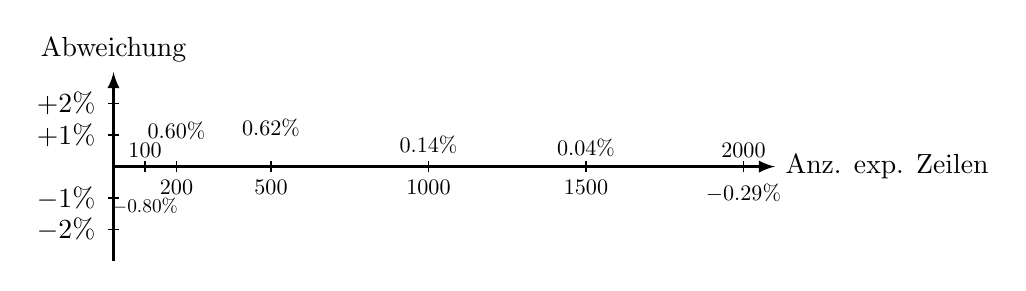
\begin{tikzpicture}[scale=0.4,>=stealth]

	%Koordinatensystem 	
	\draw[line width=1pt,>=latex,->] (0,0) -- (21,0) node[right] {Anz. exp. Zeilen};
	\draw[line width=1pt,>=latex,->] (0,-3) -- (0,3) node[above] {Abweichung};
	%Wellen einlesen und Plotten
	\draw [color=blue, thick] plot[mark=*, mark options={fill=white},ycomb] file {stosswellen/data/gauss_zeiten_abweichung.txt};
	%Beschriftung 
	\draw [line width=0.5pt] (1,-5pt) -- (1,5pt) node[scale=0.8,above=-2pt] {$100$};
	\draw [line width=0.5pt] (2,-5pt) -- (2,5pt) node[scale=0.8,below=5pt] {$200$};
	\draw [line width=0.5pt] (5,-5pt) -- (5,5pt) node[scale=0.8,below=5pt] {$500$};
	\draw [line width=0.5pt] (10,-5pt) -- (10,5pt) node[scale=0.8,below=5pt] {$1000$};
	\draw [line width=0.5pt] (15,-5pt) -- (15,5pt) node[scale=0.8,below=5pt] {$1500$};
	\draw [line width=0.5pt] (20,-5pt) -- (20,5pt) node[scale=0.8,above=-2pt] {$2000$};
	\draw [line width=0.5pt] (-5pt,1) -- (5pt,1) node[left=5pt] {$+1\%$};
	\draw [line width=0.5pt] (-5pt,-1) -- (5pt,-1) node[left=5pt] {$-1\%$};
	\draw [line width=0.5pt] (-5pt,2) -- (5pt,2) node[left=5pt] {$+2\%$};
	\draw [line width=0.5pt] (-5pt,-2) -- (5pt,-2) node[left=5pt] {$-2\%$};
	
	\node[scale=0.7,below=1pt] at (1,-0.72) {$-0.80\%$};
	\node[scale=0.8,above=1pt] at (2,0.55) {$0.60\%$};
	\node[scale=0.8,above=1pt] at (5,0.62) {$0.62\%$};
	\node[scale=0.8,above=1pt] at (10,0.09) {$0.14\%$};
	\node[scale=0.8,above=1pt] at (15,-0.02) {$0.04\%$};
	\node[scale=0.8,below=1pt] at (20,-0.24) {$-0.29\%$};
	
\end{tikzpicture}
\caption{Darstellung der prozentualen Abweichung gegen"uber der
gemittelten Programmlaufzeit pro Zeile.}
\label{stosswellen:programmabweichung}}	
\end{figure}

\subsection{Parallelisierungsansatz}
Entscheidend ist, dass die Werte $u(x, \!t \!+ \!1)$ erst berechnet werden
k"onnen, wenn alle Werte $u(x, \!t)$ bekannt sind. Aus diesem Grund
kann die Funktion zur Berechnung schlecht parallelisiert werden. Die
einzige Parallelisierungsm"oglichkeit besteht darin, das $x$-Intervall
in einzelne Teilintervalle zu unterteilen. In den Randbereichen der
Intervalle m"ussen zur Berechnung des neuen Wertes, die Werte der
Nachbarintervalle bekannt sein. Deshalb w"are auch hier eine stetige
Synchronisation der Barrier-Punkte n"otig. Die Rechenarbeit zwischen zwei
solchen Punkten betr"agt jedoch lediglich $O(n)$, was im Verh"altnis zur
Synchronisationsarbeit sehr klein ist. Aus diesem Grund lohnt sich eine
Parallelisierung im eindimensionalen Fall nicht.

Dies sieht anders aus, wenn sich die Stosswelle in mehr als einer
Dimension ausbreitet. Dann steigt die Arbeit zwischen den Barriere-Punkten
auf $O(n^{2})$ im zweidimensionalen Fall und auf $O(n^{3})$ bei drei
Dimensionen an. In diesen F"allen k"onnte man eine Zeitersparnis
gegen"uber einer sequenziellen Implementation erzielen.

\section{Visualisierung}
\lhead{Visualisierung}
Wir speichern unsere Daten in einem CSV-File ab. Diese Daten k"onnen
wir nun visualisieren. Eine einfache Methode ist, das CSV-File
in Matlab einzulesen und die Daten zu plotten wie in Abbildung
\ref{stosswellen:matlab3Dplot}. Mit Matlab k"onnen auf "ahnliche Weise
Video Dateien erzeugt werden. Die Aufl"osung der Bilder und Videos ist
von den Diskretionsschritten der Berechnung abh"angig und um Videos
fl"ussig erstellen zu k"onnen, m"ussen gen"ugend Zeilen im CSV-File
vorhanden sein. 
\begin{figure}
\begin{minipage}{0.45\textwidth}
	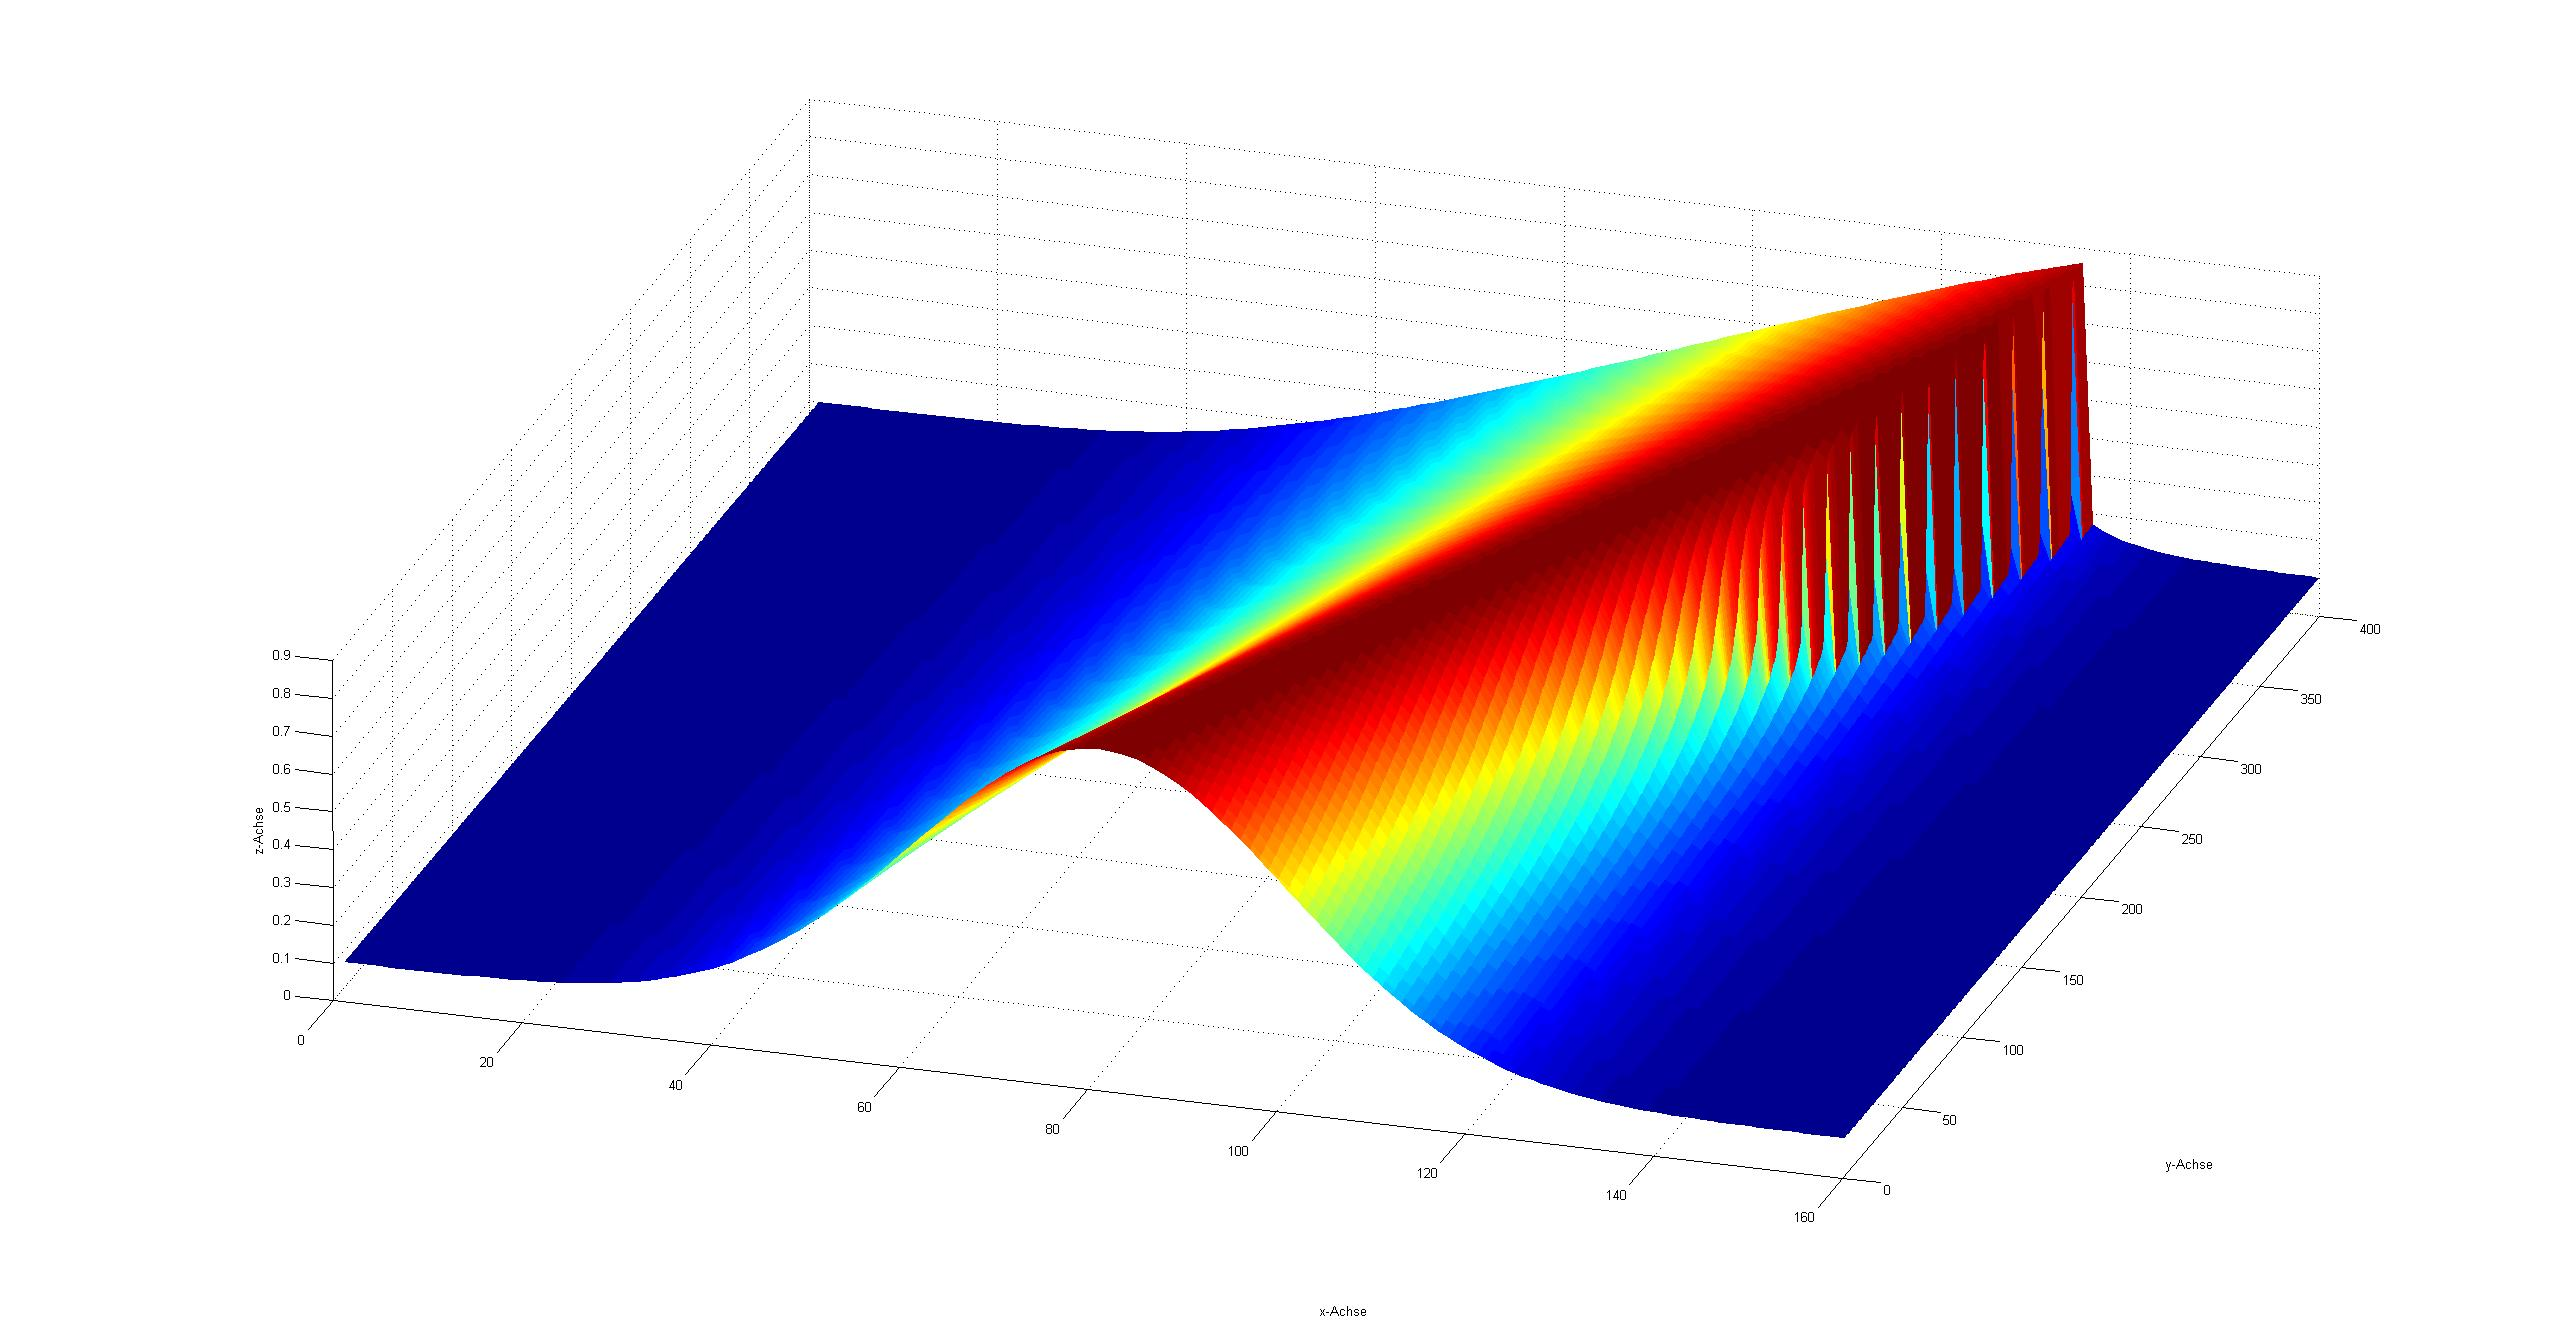
\includegraphics[width=6cm]{stosswellen/Matlab_3DPlot.jpg}
	\caption{Mit Matlab erzeugter Plot aus der CSV Datei}
\label{stosswellen:matlab3Dplot}
\end{minipage}
\hfill
\begin{minipage}{0.45\textwidth}
	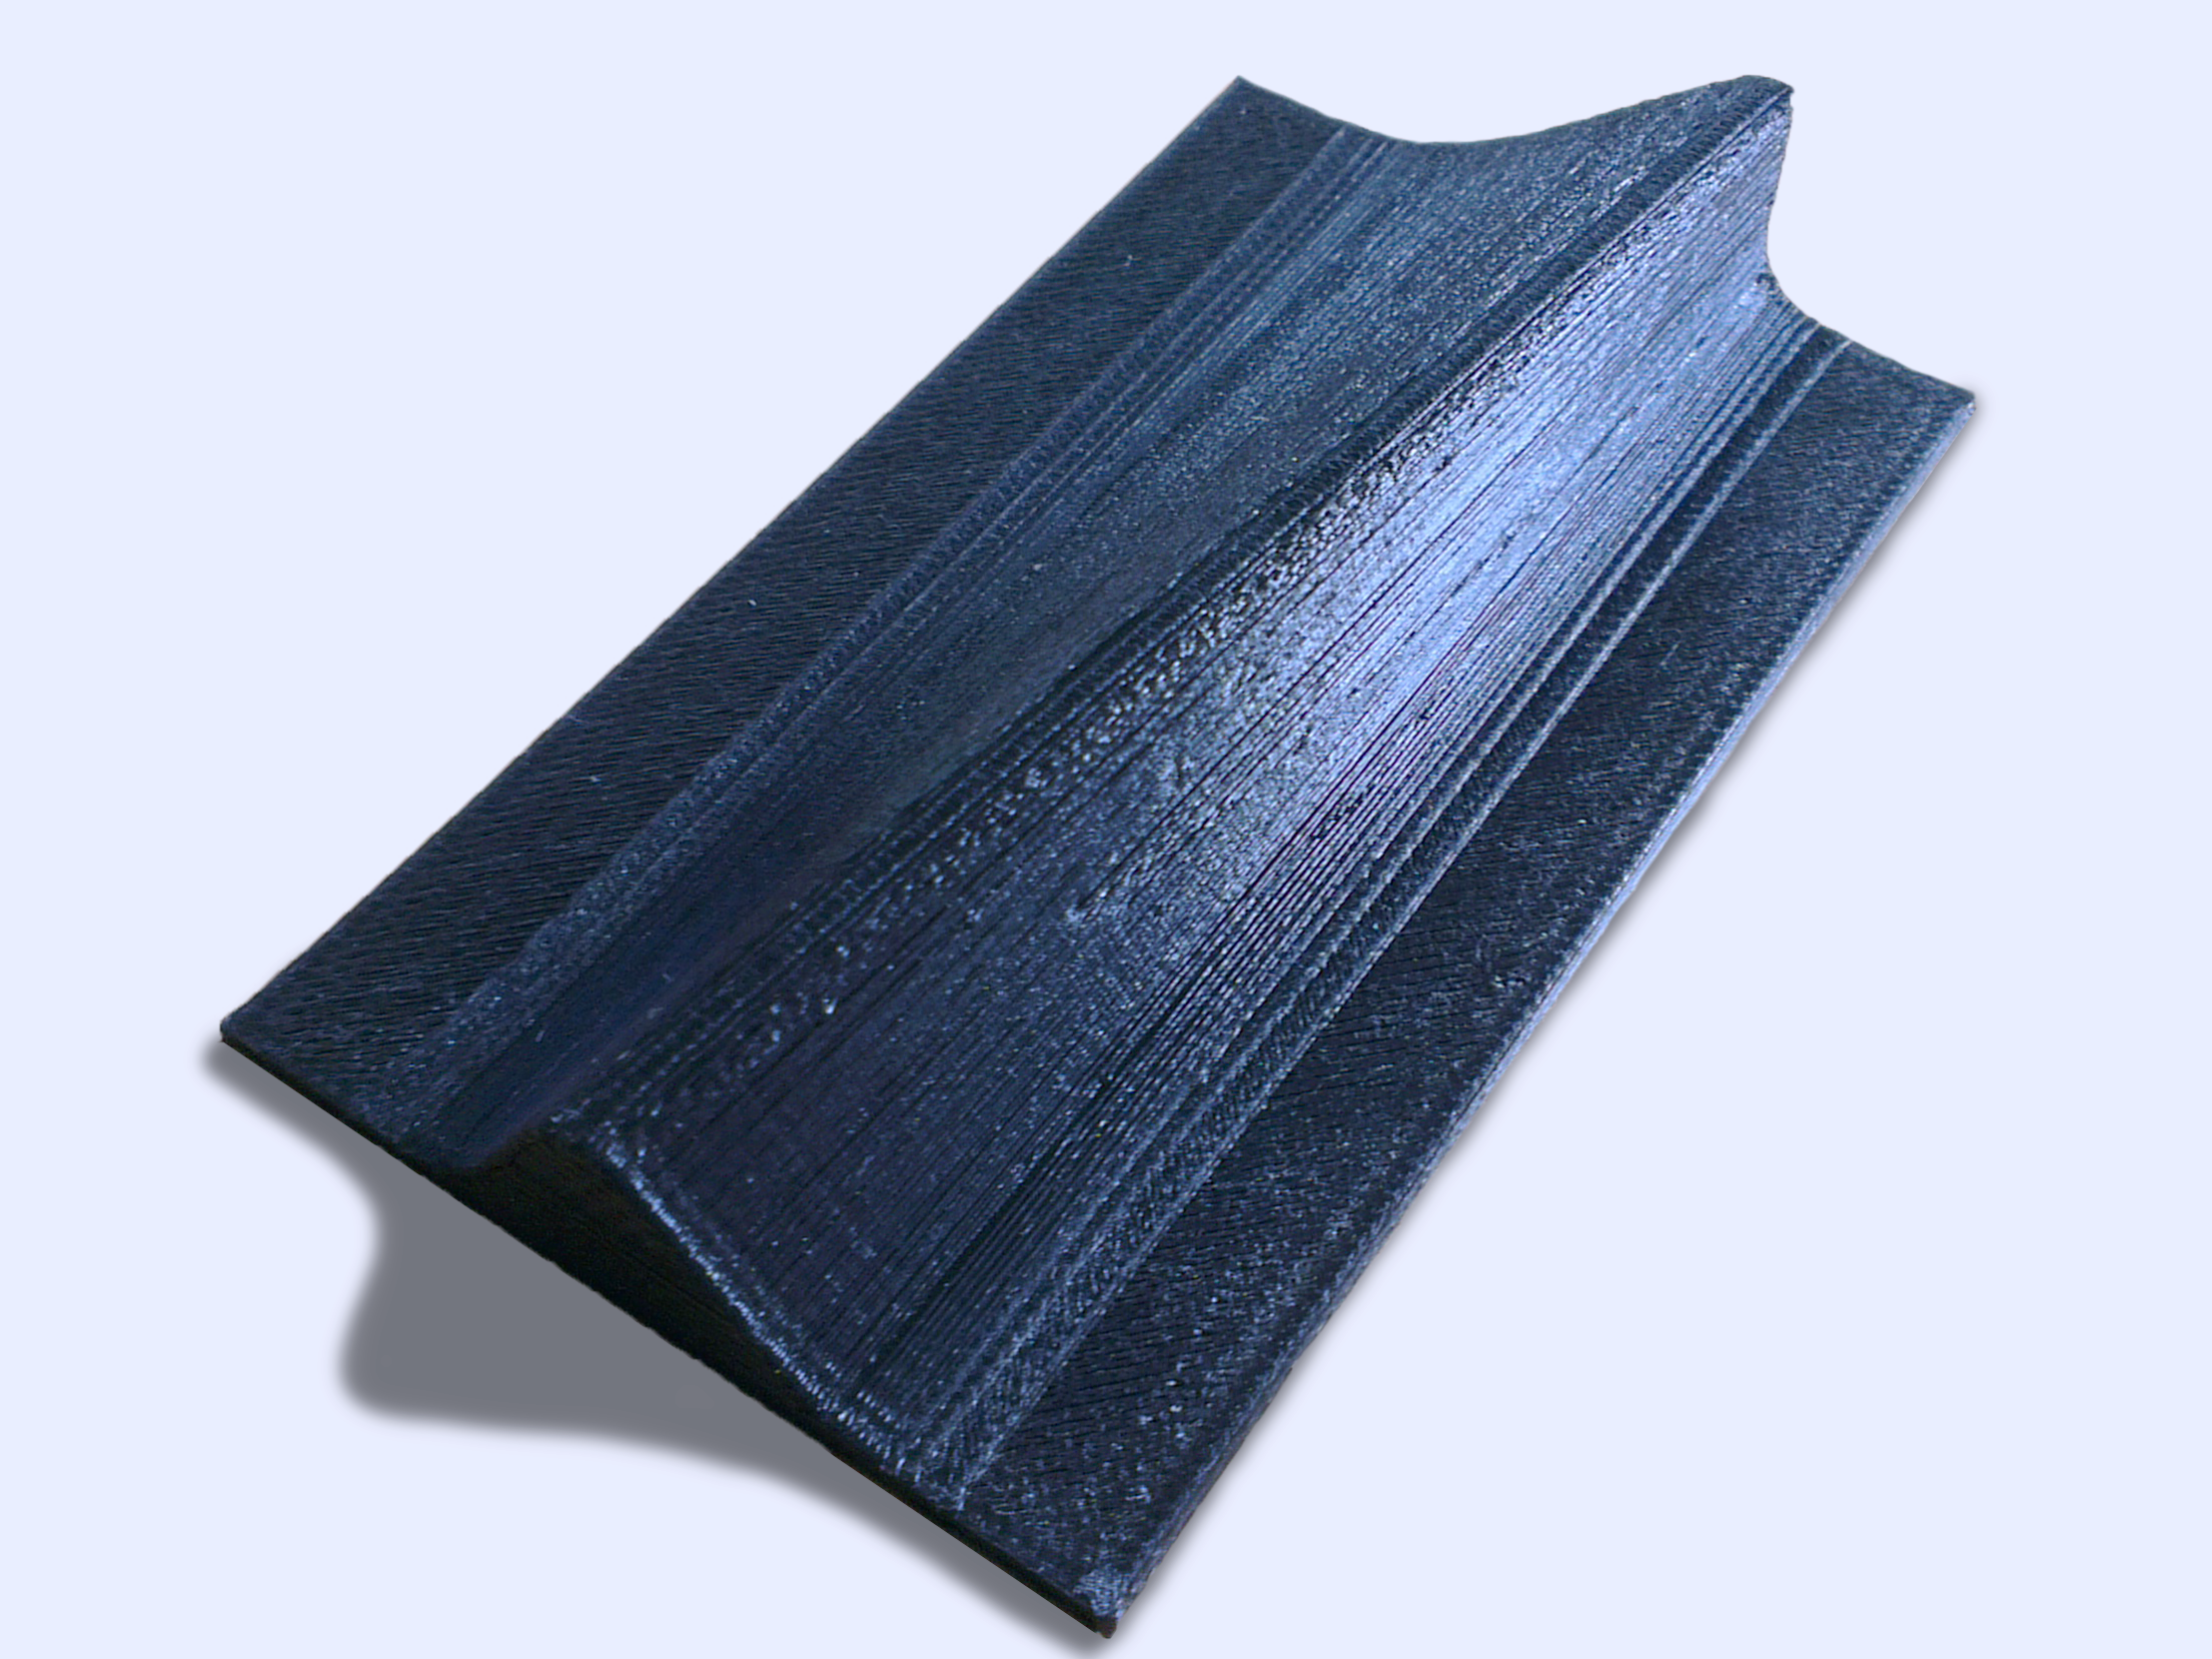
\includegraphics[width=6cm]{stosswellen/3D_print.PNG}
	\caption{3D-Druck mit einem Velleman K8200 Drucker}
	\label{stosswellen:3Dprint}
\end{minipage}
\end{figure}

Mit CAD-Programmen lassen sich die CSV-Daten in 3D-Objekte umwandeln,
sodass diese danach mit einem 3D-Drucker ausgedruckt werden k"onnen. Der
3D-Druck in Abbildung \ref{stosswellen:3Dprint} wurde mit der CAD-Software
SolidWorks und einem Velleman K8200 3D-Printer erstellt. 
\index{SolidWorks}

Um aus dem CSV-File einen 3D-K"orper erstellen zu k"onnen, gibt es
unterschiedliche Varianten. Mit zwei unterschiedlichen Methoden wurde dies
versucht, wobei schliesslich nur eine zum Erfolg f"uhrte. Bei der Ersten
werden aus der CSV-Datei einzelne Punkte gewonnen, welche anschliessend
in SolidWorks mit dem Plugin \textit{ScanTo3D} als Punktwolke eingelesen
werden k"onnen. Dieses Plugin wird normalerweise f"ur den Import von
3D-Scanndaten verwendet. Laser 3D-Scanner erzeugen durch Abtastung der
Oberfl"ache eine "ahnliche Punktwolke. 

Das Plugin ben"otig zum Import ein Textfile mit den $x$, $y$ und
$z$-Koordinaten der Punkte in nachfolgender Form, wobei $n$ der Anzahl
Elemente der urspr"unglichen Daten entspricht.
\begin{equation}
	\begin{matrix}
		x_{1}		& y_{1}		& z_{1} \\
		x_{2}		& y_{2}		& z_{2}	\\
		\vdots 		& \vdots	& \vdots\\
		x_{n}		& y _{n}	& z_{n}
	\end{matrix}
\end{equation} 

Erzeugt werden kann dieses File mit Matlab, indem das CSV-File
umsortiert wird. Alle Zeilen werden zu einer einzelnen zusammengef"ugt
und zu einem Spaltenvektor transponiert. Diese Daten entsprechen den
$y$-Koordinaten. Die $x$ und $z$-Koordinaten werden nachtr"aglich mit
einer Z"ahlschleife hinzugef"ugt. Diese $x$, $y$ und $z$-Koordinaten
repr"asentieren alle berechneten Punkte auf der Kurvenoberfl"ache. Wird
dieses File in SolidWorks importiert, entsteht eine Punktwolke wie in
Abbildung \ref*{stosswellen:pointcloud}.
\begin{figure}
\begin{minipage}{0.45\textwidth}
	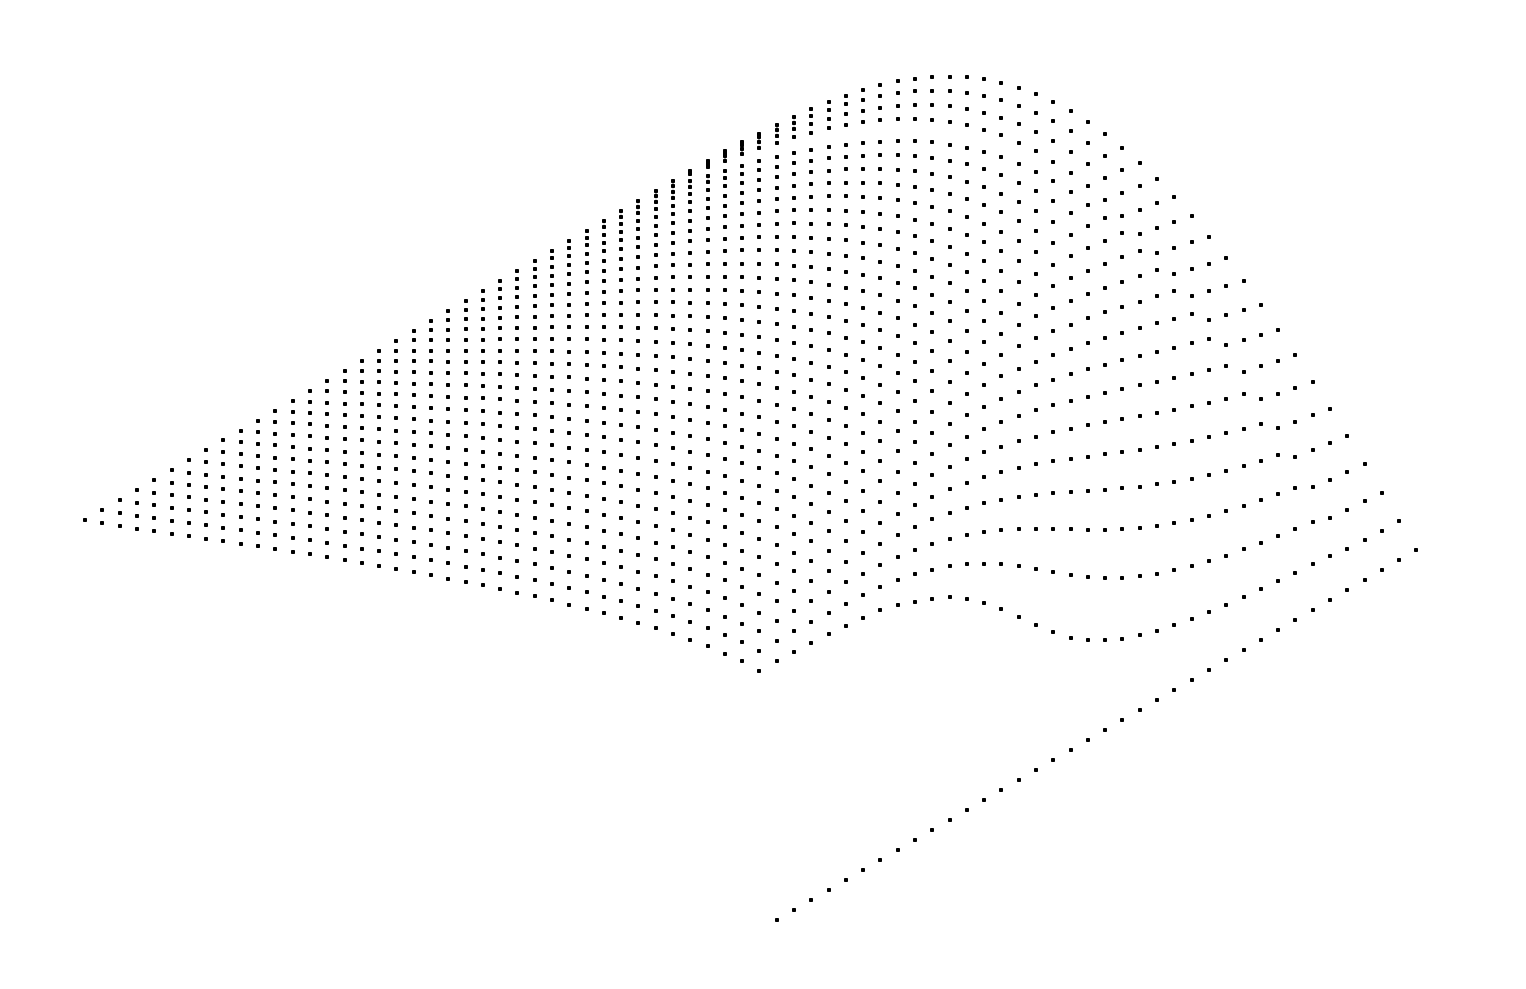
\includegraphics[width=6cm]{stosswellen/pointCloud.PNG}
	\caption{Punktwolke in SolidWorks}
\label{stosswellen:pointcloud}
\end{minipage}
\hfill
\begin{minipage}{0.45\textwidth}
	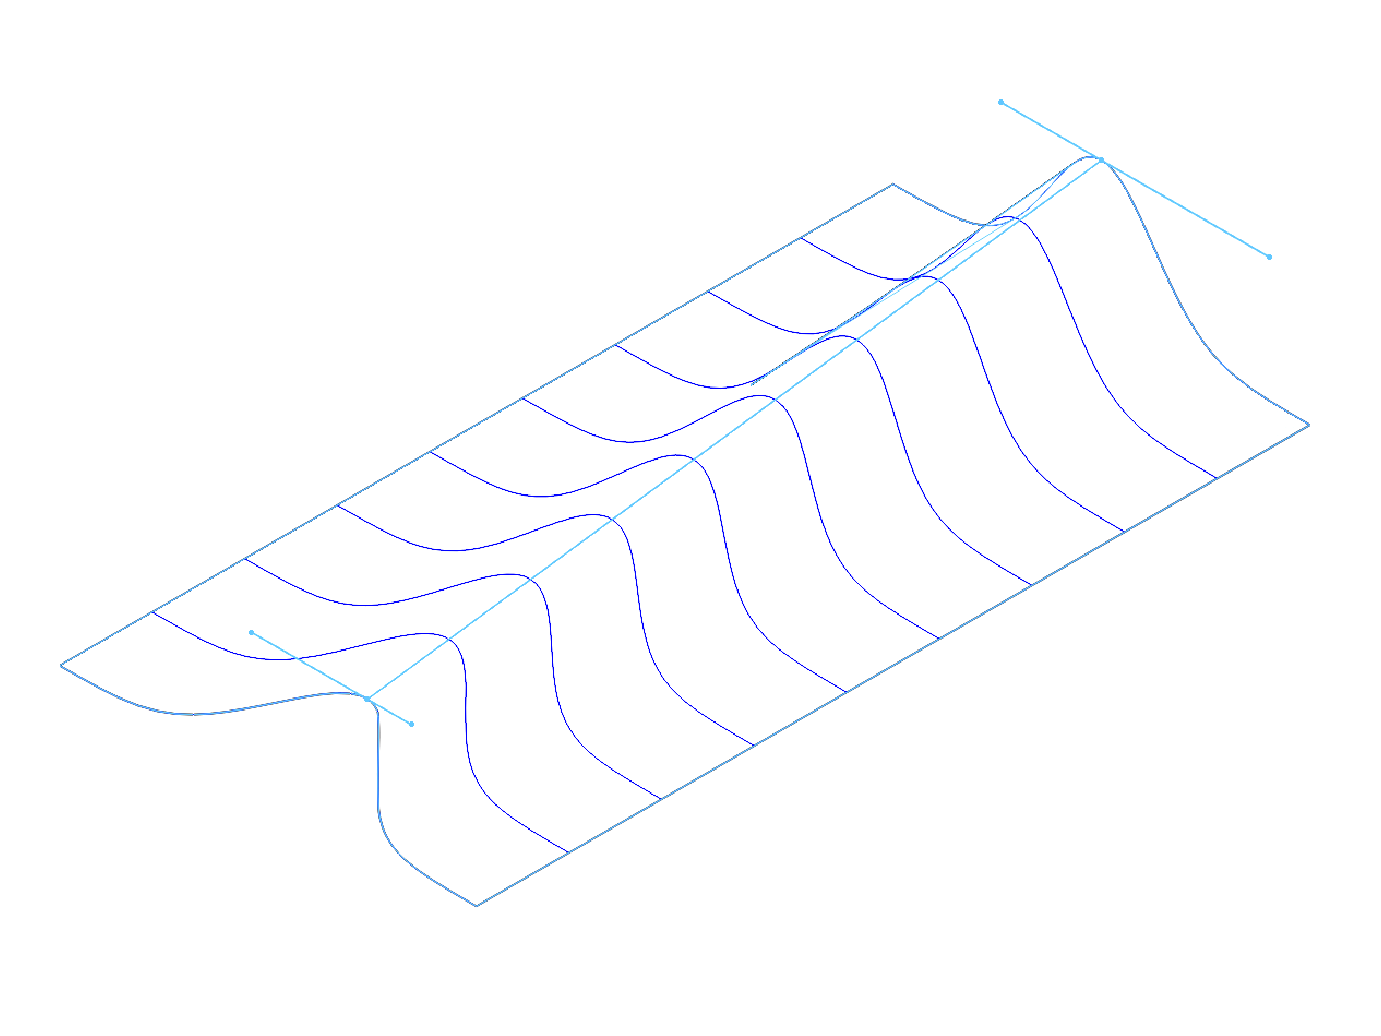
\includegraphics[width=6cm]{stosswellen/importedCurves.PNG}
	\caption{Importierte Kurven durch Punkte in SolidWorks}
	\label{stosswellen:importedCurves}
\end{minipage}
\end{figure}

Es entsteht nun ein Problem bei den Sprungstellen. Da die Punkte an diesen
Stellen zu weit auseinanderliegen, erkennt SolidWorks diese Punkte nicht
automatisch als benachbarte, sie k"onnen dadurch nicht mit einer Fl"ache
verbunden werden. Um einen K"orper zu erhalten muss jedoch eine Fl"ache
vorhanden sein, welche ausgetragen werden kann. 

Die zweite M"oglichkeit, welche im Fall der Stosswelle einfacher
zu handhaben ist, ist der Import von einzelnen Kurven. Aus dem
CSV-File werden nicht mehr alle, sondern nur noch ein paar Zeilen in
regelm"assigen Abst"anden ben"otigt. Eine Zeile wird in analoger Weise
wie bei der Punktwolke in ein File mit $x$, $y$ und $z$-Koordinaten
exportiert. Beim Import in SolidWorks wird jedoch das Feature
\textit{Curve Through XYZ Points} verwendet und alle Files nacheinander
eingelesen (in diesem Fall 10 St"uck). In der nachfolgenden Abbildung
\ref{stosswellen:importedCurves} sind die importierten, einzelnen Kurven
zu sehen. Ebenfalls zu erkennen ist, dass an den Sprungstellen durch
dieses Feature die Punkte verbunden werden und kein Loch entsteht. 

Mit einer Hilfslinie entlang der Scheitelpunkte (zu sehen in Abbildung
\ref{stosswellen:importedCurves}) kann nun eine Fl"ache erzeugt werden,
welche die Kurven verbindet. Zur Erzeugung eines K"orpers, kann diese
Oberfl"ache auf die Grundfl"ache ausgetragen werden, wobei ein K"orper
wie in Abbildung \ref{stosswellen:solid} entsteht.
\begin{figure}
	\begin{center}
		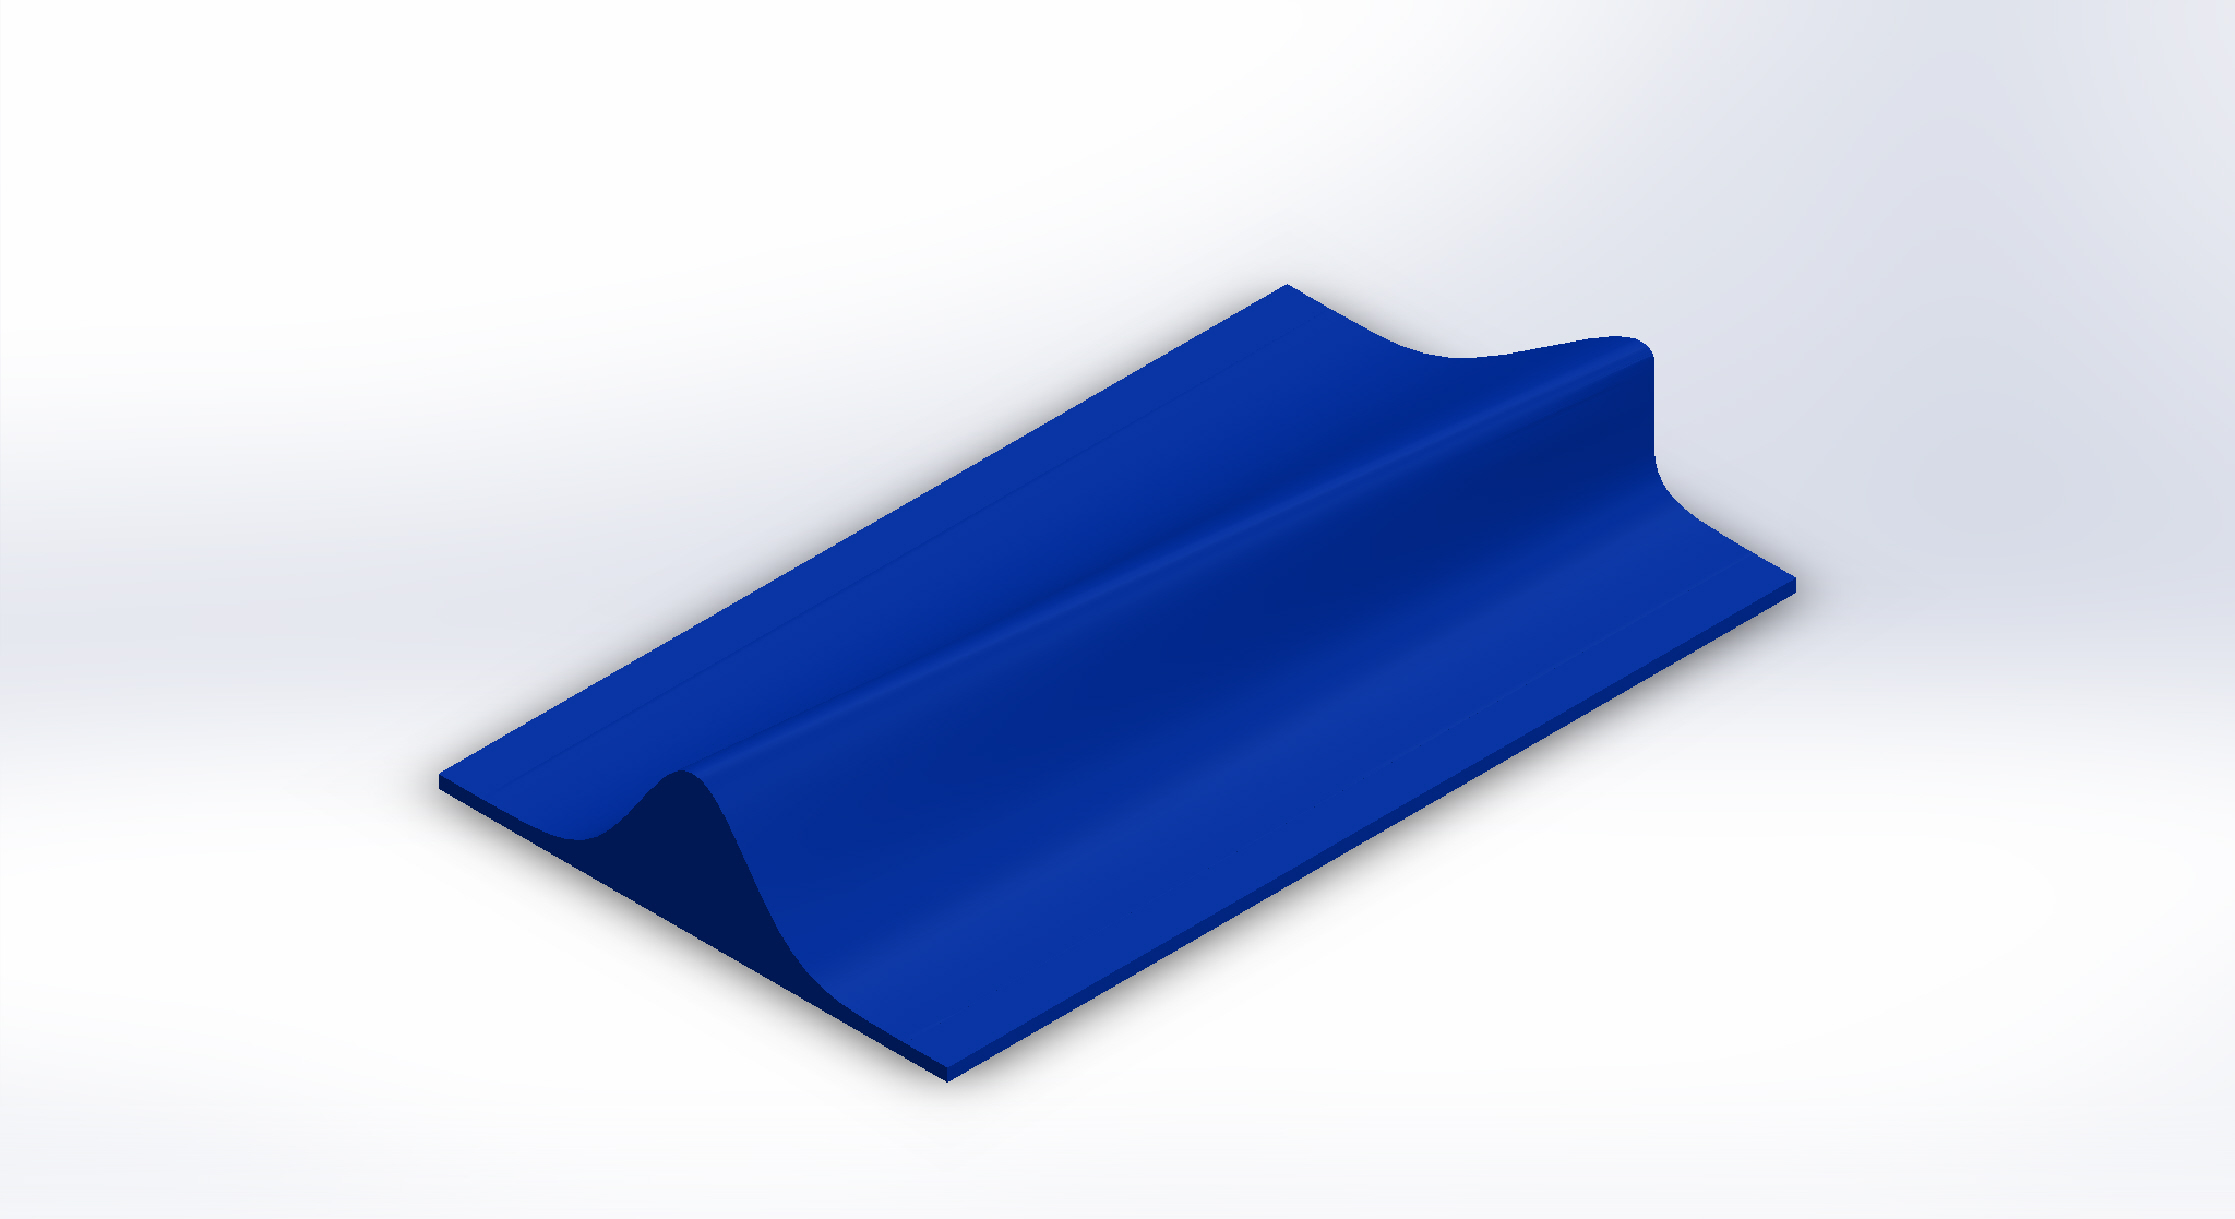
\includegraphics[width=8cm]{stosswellen/Solid.JPG}
	\end{center}
	\caption{Ausgetragener K"orper von der Oberfl"ache zur Grundfl"ache}
\label{stosswellen:solid}
\end{figure}

Dieser K"orper kann als .STL File exportiert und zum Druck verwendet
werden. 
Der verwendete 3D-Printer ist ein K8200 von Velleman mit der
\index{3D-Printer}
Standart Open-Source Software \textit{RepetierHost} zur Erzeugung
der Druckdaten. Der fertiggestellte Druck ist in Abbildung
\ref{stosswellen:3Dprint} zu sehen.
\printbibliography[heading=subbibliography]
\end{refsection}
